\documentclass[10pt, xcolor=dvipsnames]{beamer}

\usetheme{metropolis}
\usepackage[utf8]{inputenc}
\usepackage[english]{babel}
\usepackage{ragged2e}
\usepackage{bbding}
%\usepackage{enumitem}
\usepackage{mathtools}
\usepackage{indentfirst}
\usepackage{graphicx}
\usepackage{float}
\usepackage{hyperref}
\usepackage{mathtools}
\usepackage{preview}
\usepackage{xcolor}
\usepackage{color}
\usepackage{listings}
\usepackage{float}
\usepackage[caption = false]{subfig}
\usepackage{pdfpages}
\usepackage{multirow}
\usepackage{array}
\usepackage{makecell}
\usepackage{bm}
\usepackage{caption}
\usepackage{cancel}
\usepackage{anyfontsize}
\usepackage{etoolbox}
\usepackage{mathtools}
\usepackage{subcaption}
\usepackage[flushleft]{threeparttable}
\usepackage{booktabs}
\usepackage{caption}
\usepackage{adjustbox}
\usepackage{appendixnumberbeamer}
\usepackage{pifont}
\usepackage{amsmath}
\usepackage{amssymb}
\usepackage[percent]{overpic}

%\usepackage{biblatex}
\usepackage[backend=biber,
style=authoryear,
citestyle=authoryear]{biblatex} 
\addbibresource{latex/bibliography.bib}

\setbeamercolor{titlelike}{parent=structure}
\definecolor{UBCblue}{rgb}{0.04706, 0.13725, 0.32}
\colorlet{UBCblue2}{UBCblue!70!white}
\usecolortheme[named=UBCblue]{structure}

\makeatletter
\setbeamertemplate{footline}
{
  \leavevmode%
  \hbox{%
  \begin{beamercolorbox}[wd=.4\paperwidth,ht=2.25ex,dp=1ex,center]{author in head/foot}%
    \usebeamerfont{author in head/foot} \insertshortauthor %\hspace*{1em}(\insertshortinstitute)
  \end{beamercolorbox}%
  \begin{beamercolorbox}[wd=.5\paperwidth,ht=2.25ex,dp=1ex,center]{title in head/foot}%
    \usebeamerfont{title in head/foot} \insertshorttitle
  \end{beamercolorbox}%
  \begin{beamercolorbox}[wd=.1\paperwidth,ht=2.25ex,dp=1ex,center]{date in head/foot}%
    \usebeamerfont{date in head/foot}
    \insertframenumber{} / \inserttotalframenumber\hspace*{2ex} 
  \end{beamercolorbox}}%
  \vskip0pt%
}
\makeatother

\renewcommand{\arraystretch}{1.2}
\renewcommand{\raggedright}{\leftskip=0pt \rightskip=0pt plus 0cm}
\newcolumntype{C}[1]{>{\centering\let\newline\\\arraybackslash\hspace{0pt}}m{#1}}

\hypersetup{
    colorlinks=true,
    linkcolor=UBCblue,
    citecolor=UBCblue,
    filecolor=magenta,      
    urlcolor=blue,
    allcolors=.
}

\setbeamercolor{button}{bg=UBCblue2,fg=white}
\newcommand\fnote[1]{\captionsetup{font=tiny}\caption*{#1}}
\newcommand\fnotev[1]{\captionsetup{font=scriptsize}\caption*{#1}}
\def\house{\hbox{\kern3pt \vbox to13pt{}% 
   \pdfliteral{q 0 0 m 0 5 l 5 10 l 10 5 l 10 0 l 7 0 l 7 5 l 3 5 l 3 0 l f
               1 j 1 J -2 5 m 5 12 l 12 5 l S Q }%
   \kern 13pt}}
\setbeamertemplate{caption}[numbered]
\setbeamertemplate{itemize item}{\Tiny \house}
\metroset{progressbar=frametitle,numbering=fraction}
% %\justifying
% \urlstyle{same}
%\usefonttheme{serif}

%\usefonttheme{serif}

%------------------------
%------------------------

\date{}

%------------------------
%------------------------
%----------------------------------------------------------------------------------------
%	TITLE PAGE
%----------------------------------------------------------------------------------------------------------------
%------------------------

\title[Landlord Responses to Changes in Tenant Protections]{Optimal Slumlord Regulation: \\Landlord Responses to Changes in Tenant Protections} % The short title appears at the bottom of every slide, the full title is only on the title page
\author[Joe Fish]{Joe Fish}


\begin{document}

\begin{frame}
\titlepage % Print the title page as the first slide
\end{frame}

\begin{frame}{Motivation}
    \begin{enumerate}
        \item About 80\% of low income renters live in private market units \parencite{jchs_2024, nhpd2024profiles}
        \pause
        \item Low income landlords are both more punitive (lower threshold to evict) and more profitable \parencite{Desmond_2019, Eisfeldt_2015,Damen_2025}
        \item Evictions have large personal and social cost \parencite{desmond-evicted,humphries2025, collison-et-al-2023}
        \begin{itemize}
            \item Suggests room to regulate the worst landlords
        \end{itemize}
        \pause
        \item At the same time, given reliance on private market and lack of funds for subsidized housing, optimal regulation has to be careful about inducing landlord exit
        \begin{itemize}
            \item Optimal regulation requires the distribution of exit/upgrade options across landlords
        \end{itemize}
    \end{enumerate}

\end{frame}


\begin{frame}{Questions of Interest}
    \begin{itemize}
        \item How do landlords respond to changes in tenant protections?
        \begin{itemize}
           \item Case study of overhaul of eviction process in Philadelphia, PA
        \end{itemize}
         \item How do landlord responses vary by market position, outside option, idiosyncratic costs, etc.?
         \item Given landlord response function, what does optimal regulation look like?
         \item Equilibrium implications under counterfactual policy designs
    \end{itemize}
\end{frame}

\begin{frame}{This Presentation}
    \begin{enumerate}
        \item Background on Philadelphia rental market, eviction diversion program, and right to counsel
        \item Toy model of landlord response to change in tenant protections
        \item Nested logit of market segmentation
        %\item Reduced form evidence of changes in landlord behavior (pricing, maintenance)
    \end{enumerate}
    
\end{frame}

\begin{frame}{Desired Feedback}
    \begin{itemize}
        \item Framing / positioning in the literature
        \item Model, both theoretical and how I might estimate parts of it
        \item Tips on demand estimation
    \end{itemize}
    
\end{frame}

\begin{frame}{Existing Literature}
    \textbf{Rent Control}
    \begin{itemize}
        \item Studies on price effects \cite{diamond-2019, Jofre_Monseny_2023, Kholodilin_2024}
        \item Studies on housing quality \cite{Gyourko_1990 }
    \end{itemize}
    \textbf{Tenant Protections}
    \begin{itemize}
        \item \cite{humphries-2024}: Looks at how landlords respond to a change in tenant protections in NYC; finds price pass through onto tenants
        \item \cite{abramson_2021, Asquith_2019, Corbae_2024} 
    \end{itemize}
    
\end{frame}


\section{Data}

\begin{frame}{Data}
\textbf{Eviction Data}
    \begin{itemize}
        \item Universe of Eviction Records from 2006-2025
        \begin{itemize}
            \item Contain \textbf{contract rents} as well case information (address, amount owed, plaintiff / defendant name, etc.)
            \item Cases are filtered to non-commercial and non-housing authority
        \end{itemize}
    \end{itemize}
\pause
\textbf{Rental listing data from Altos (2011-2023)}
\begin{itemize}
    \item Unit level rental listings with information on amenities, beds, baths, etc.
\end{itemize}
\textbf{ Rental Registry}
\begin{itemize}
    \item Covers near-universe of rental listings
    \item Importantly, landlords need to be on the rental listing to file evictions
\end{itemize}
\textbf{Address History Data from Infutor}
    \pause
Why this is important:\\
    \begin{itemize}
        \item This will be one of the few papers to study the low income rental market because data are so sparse 
    \end{itemize}
\end{frame}

\begin{frame}{Distribution of Rent Prices by Data Source}
Commercially available rental datasets (\textcolor{red}{altos}) don't cover the low income rental market\\
    \begin{figure}
        \centering
        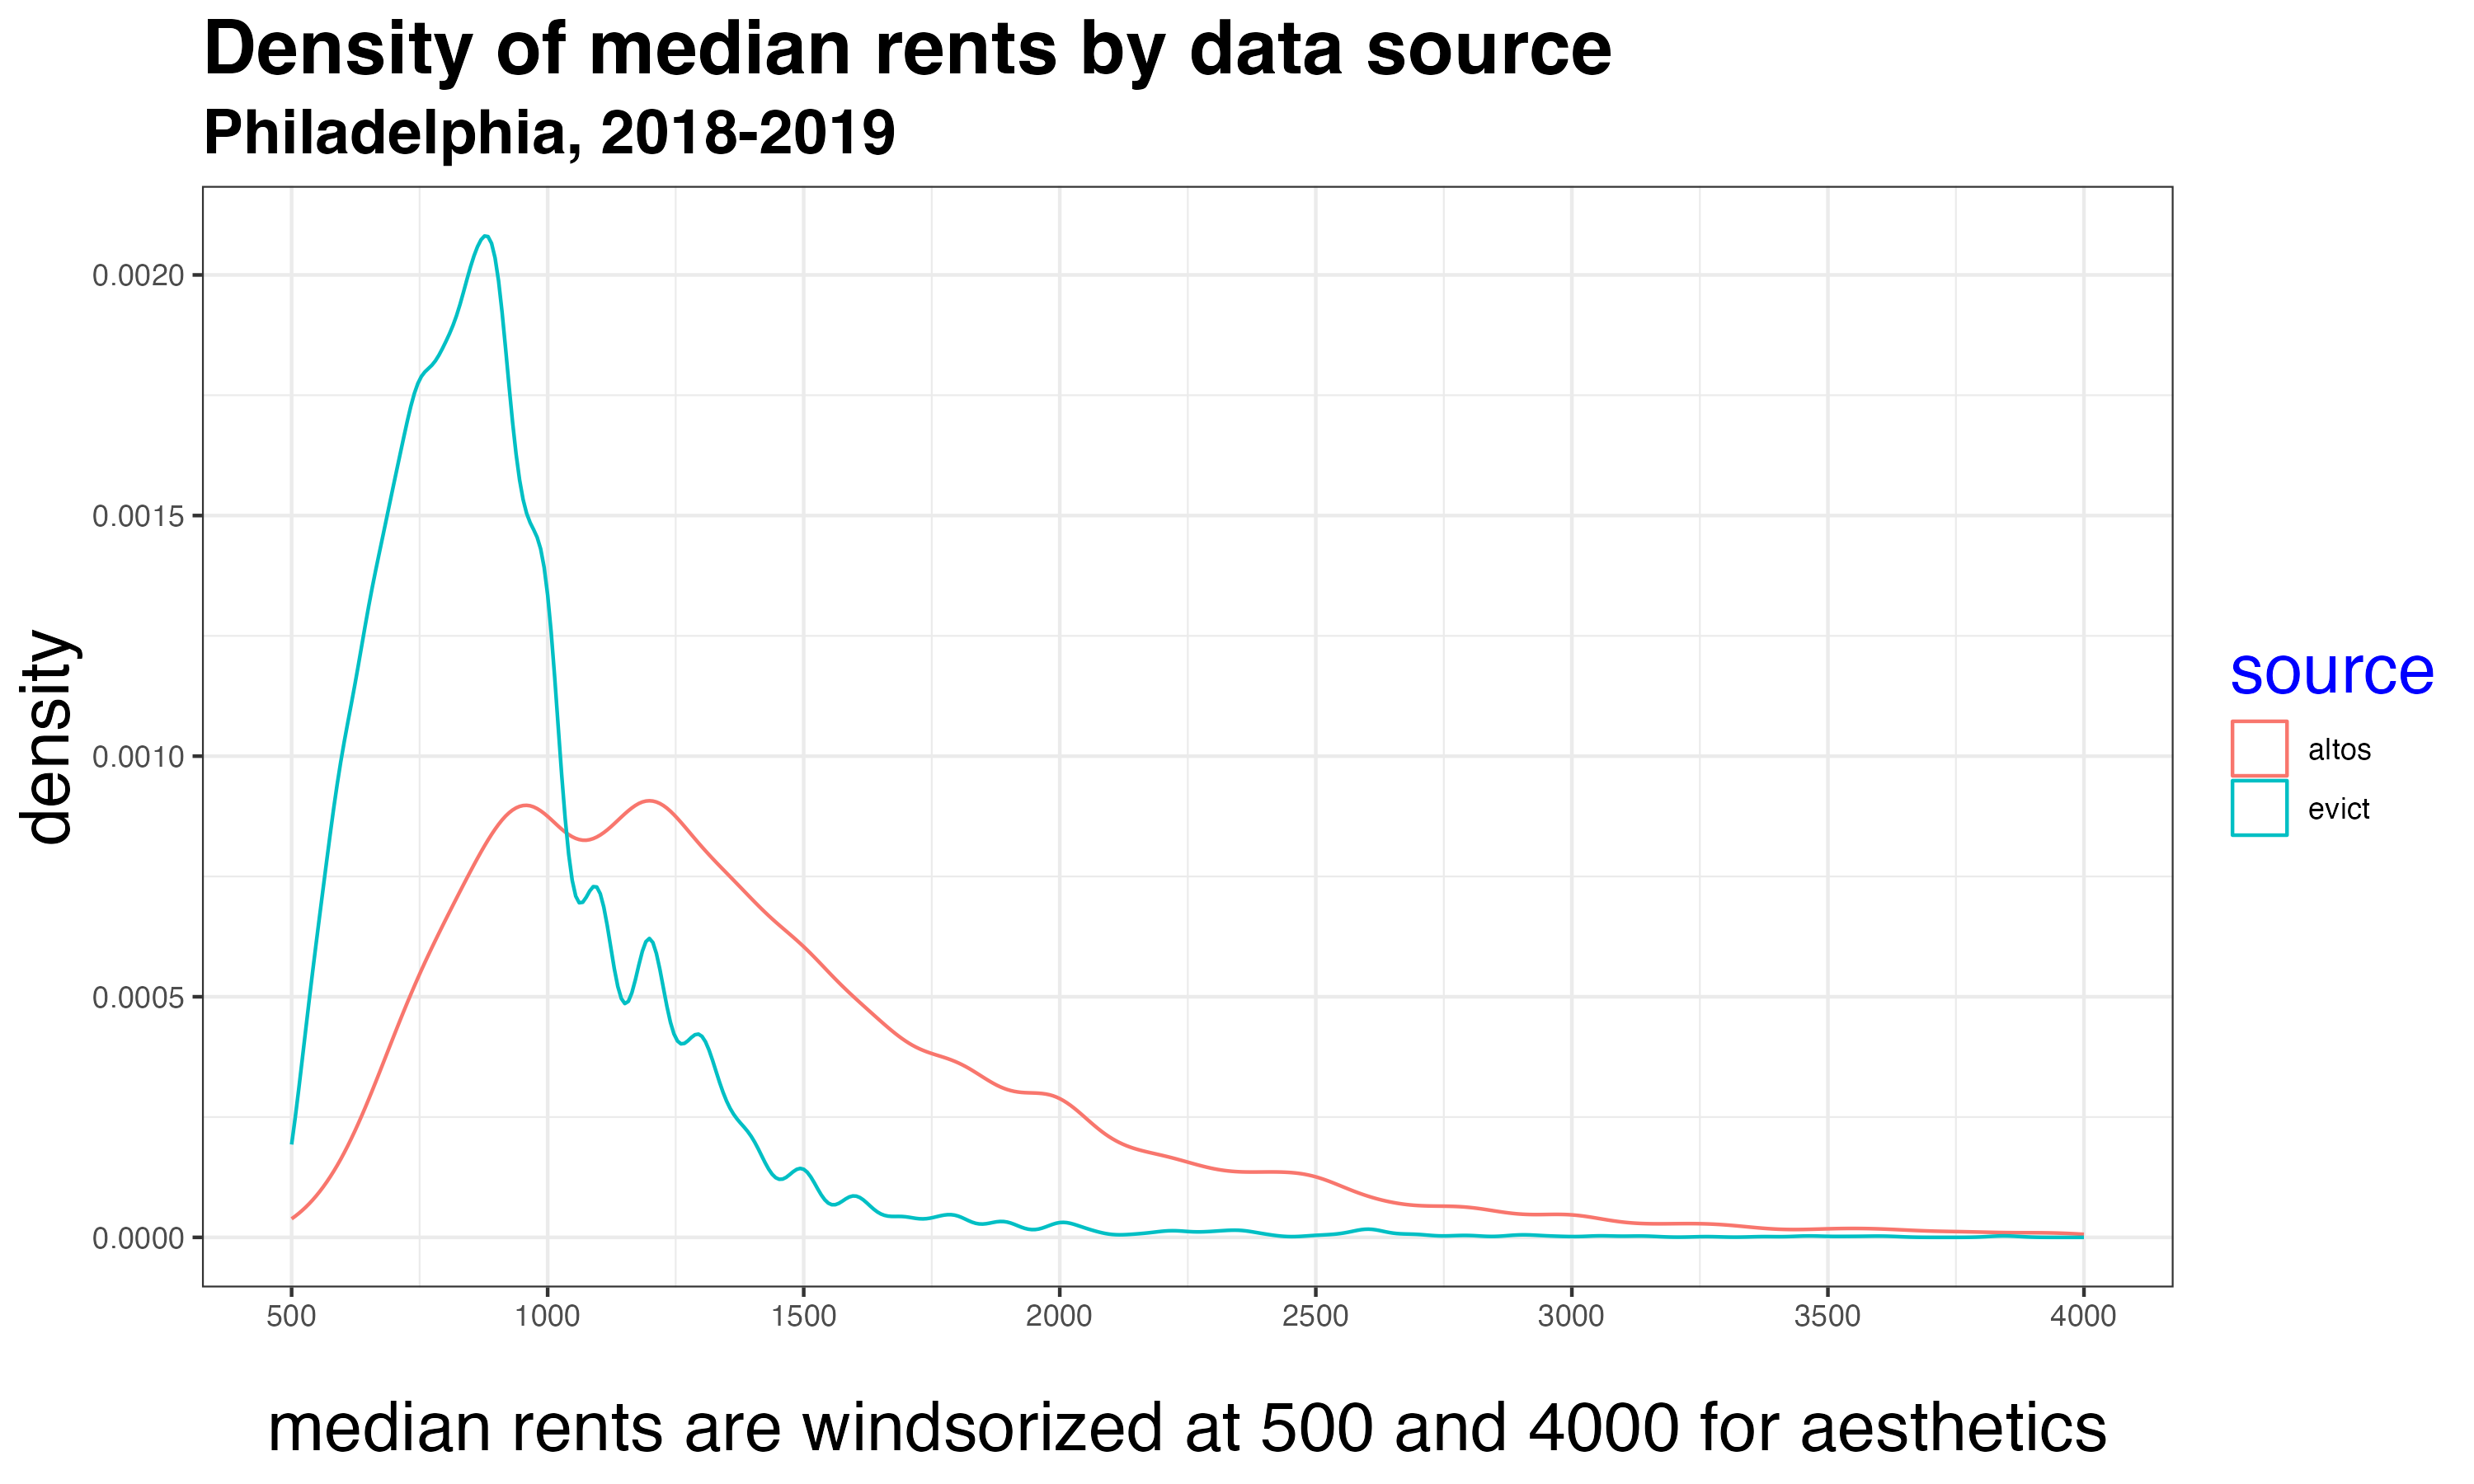
\includegraphics[width=0.75\linewidth]{figs/density_rent_prices.png}
        \caption{Rent Prices by Data Source}
        \label{fig:rent-dist}
    \end{figure}
\end{frame}

\section{Setting and Context}
\begin{frame}{Common Ways of Regulating Eviction}
    \textbf{Fee cost shifters}
    \begin{itemize}
        \item Filing Fees: Increase marginal cost of filing eviction
        \item Longer notice periods
    \end{itemize}
    \textbf{Win-probability/time-to-vacancy shifters}
    \begin{itemize}
        \item Right to Counsel
    \begin{itemize}
        \item Decreases probability of winning an eviction case, conditional on filing; increases amount of time tenant can stay in unit following default; decreases amount tenant pays to landlord
    \end{itemize}
    \end{itemize}
    \textbf{General Legal Climate}
    \begin{itemize}
        \item Good cause eviction ordinances
        \item Restrictions on landlord exit
        \item Allowable reasons for tenants to withhold rent
    \end{itemize}
    
    
\end{frame}

\begin{frame}{Stylized Facts on Eviction in Philadelphia}
    \begin{itemize}
        \item Eviction is relatively infrequent
        \item A small share of properties have very high eviction rates
    \end{itemize}

    \begin{figure}
        \centering
        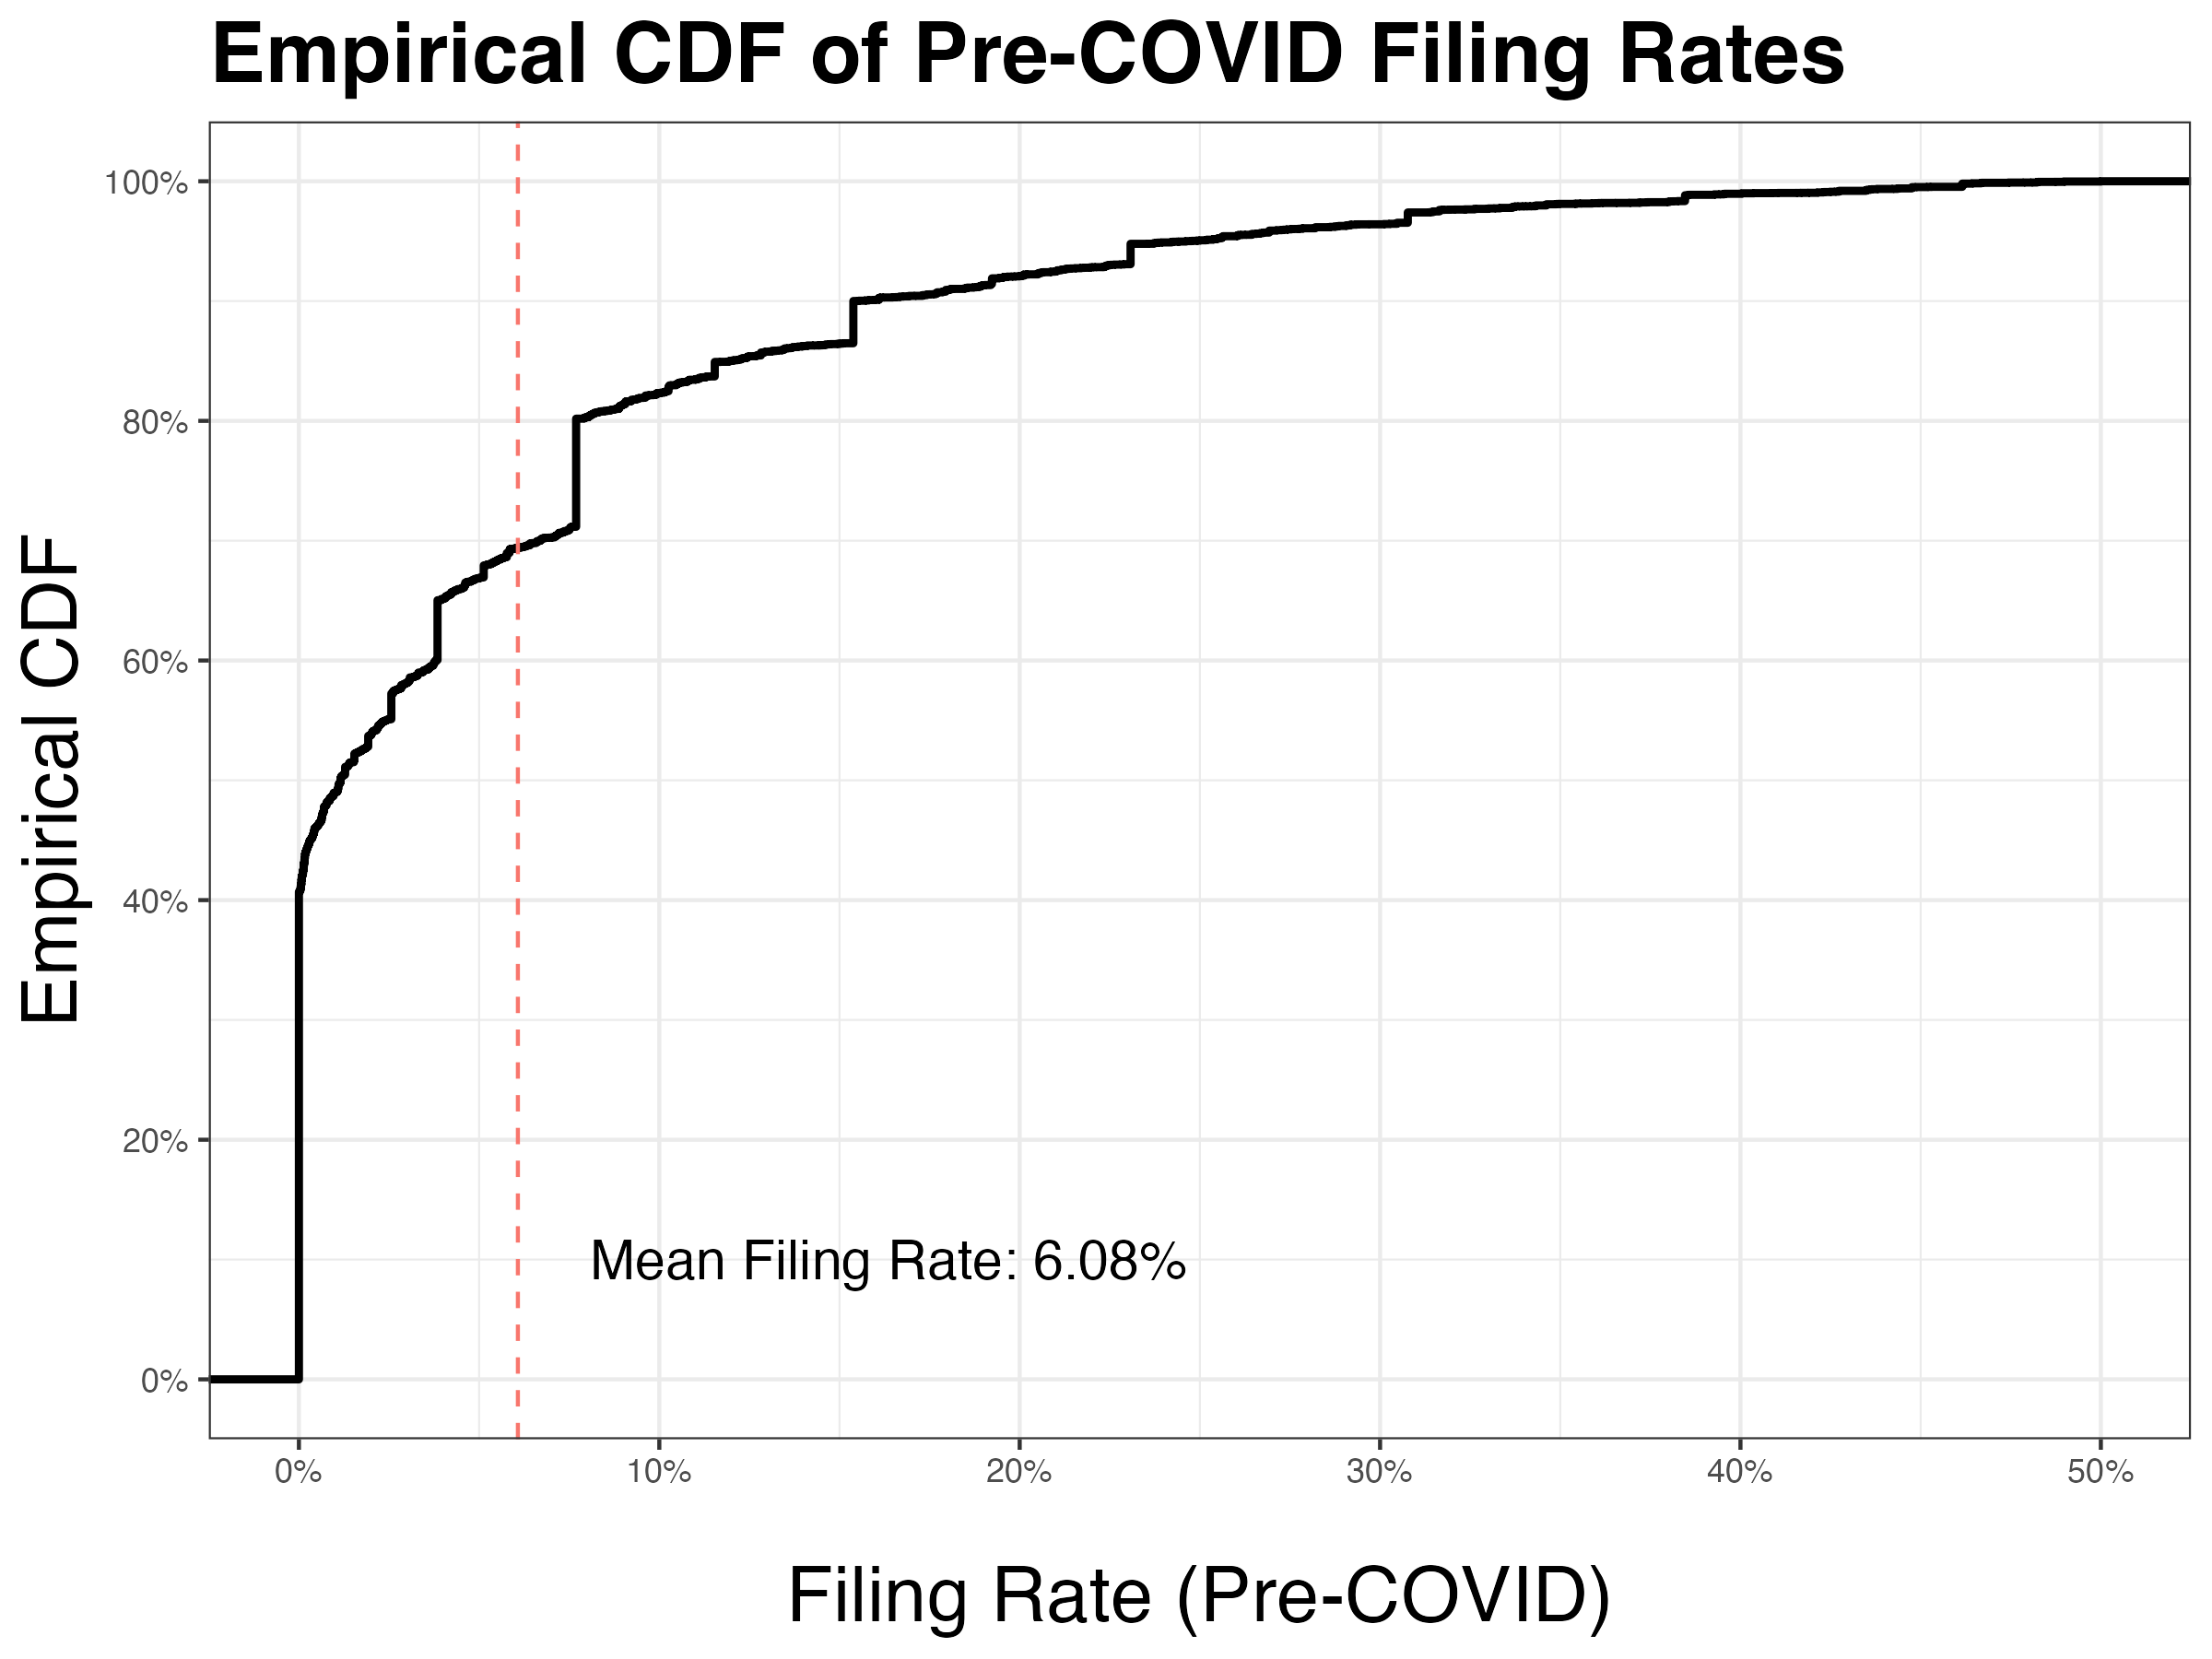
\includegraphics[width=0.75\linewidth]{figs/empirical_cdf_filing_rate_preCOVID.png}
        \caption{Empirical CDF of Filing Rate (pre-COVID)}
        \label{fig:ecdf-filings}
    \end{figure}
    
\end{frame}

\begin{frame}{Evictions in Philadelphia}
    \begin{figure}
        \centering
        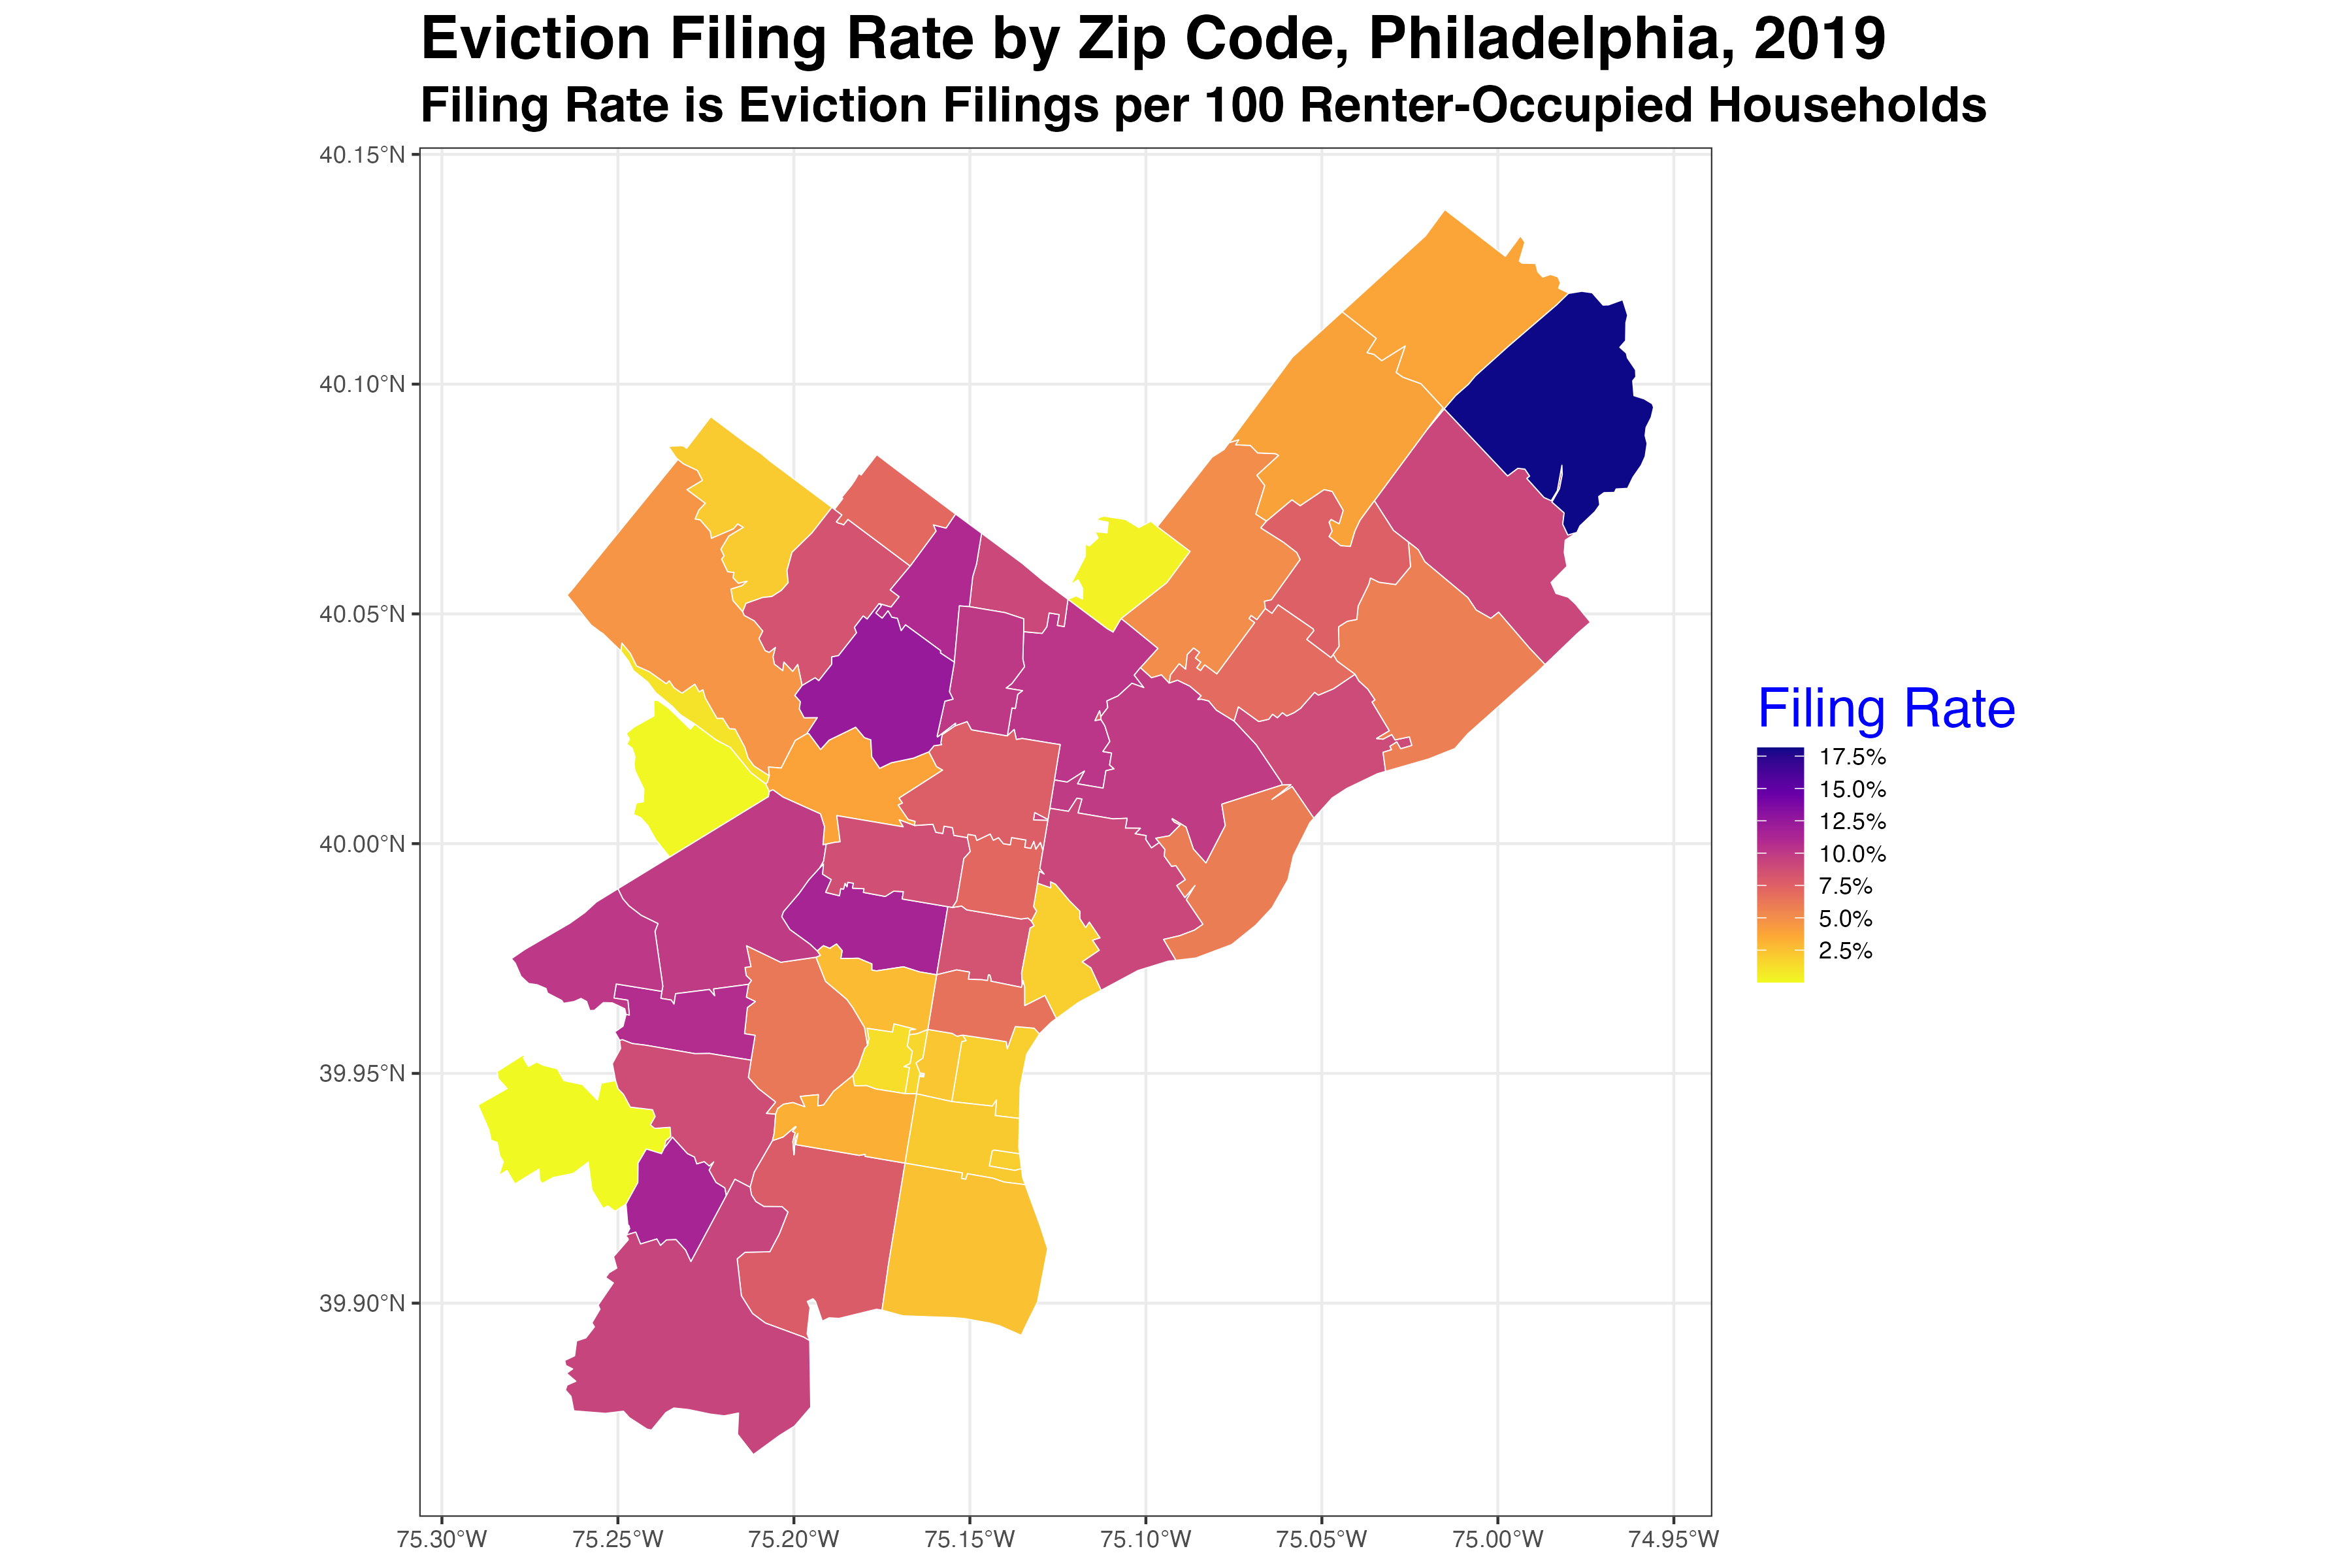
\includegraphics[width=0.75\linewidth]{figs/pa_zip_filing_rate_2019.png}
        \caption{Filing Rates by Philadelphia Zip Code}
        \label{fig:philly-zip}
    \end{figure}
\end{frame}


\begin{frame}{Philadelphia's Eviction Diversion Program}
    \begin{itemize}
        \item Announced in 2020, implemented in 2021 (alongside expiration of moratorium)
        \item Law required all landlords to apply and be approved for the Eviction Diversion Program and participate in good faith for at least 30 days before filing an eviction in court
        \item Depending on the application, the landlord either bargains directly with the tenant or with a tenant and a mediator
        \item if bargaining breaks down, landlord can file an eviction and proceed to court
    \end{itemize}

    Eviction diversion raises the cost of filing an eviction, but can lower the cost of removing a tenant (anecdotally, landlords report higher overall costs). On the tenants' side, eviction diversion prevents an eviction from appearing on their record.
\end{frame}

\begin{frame}{Effectiveness of Philadelphia's Eviction Diversion Program}
    \begin{figure}
        \centering
        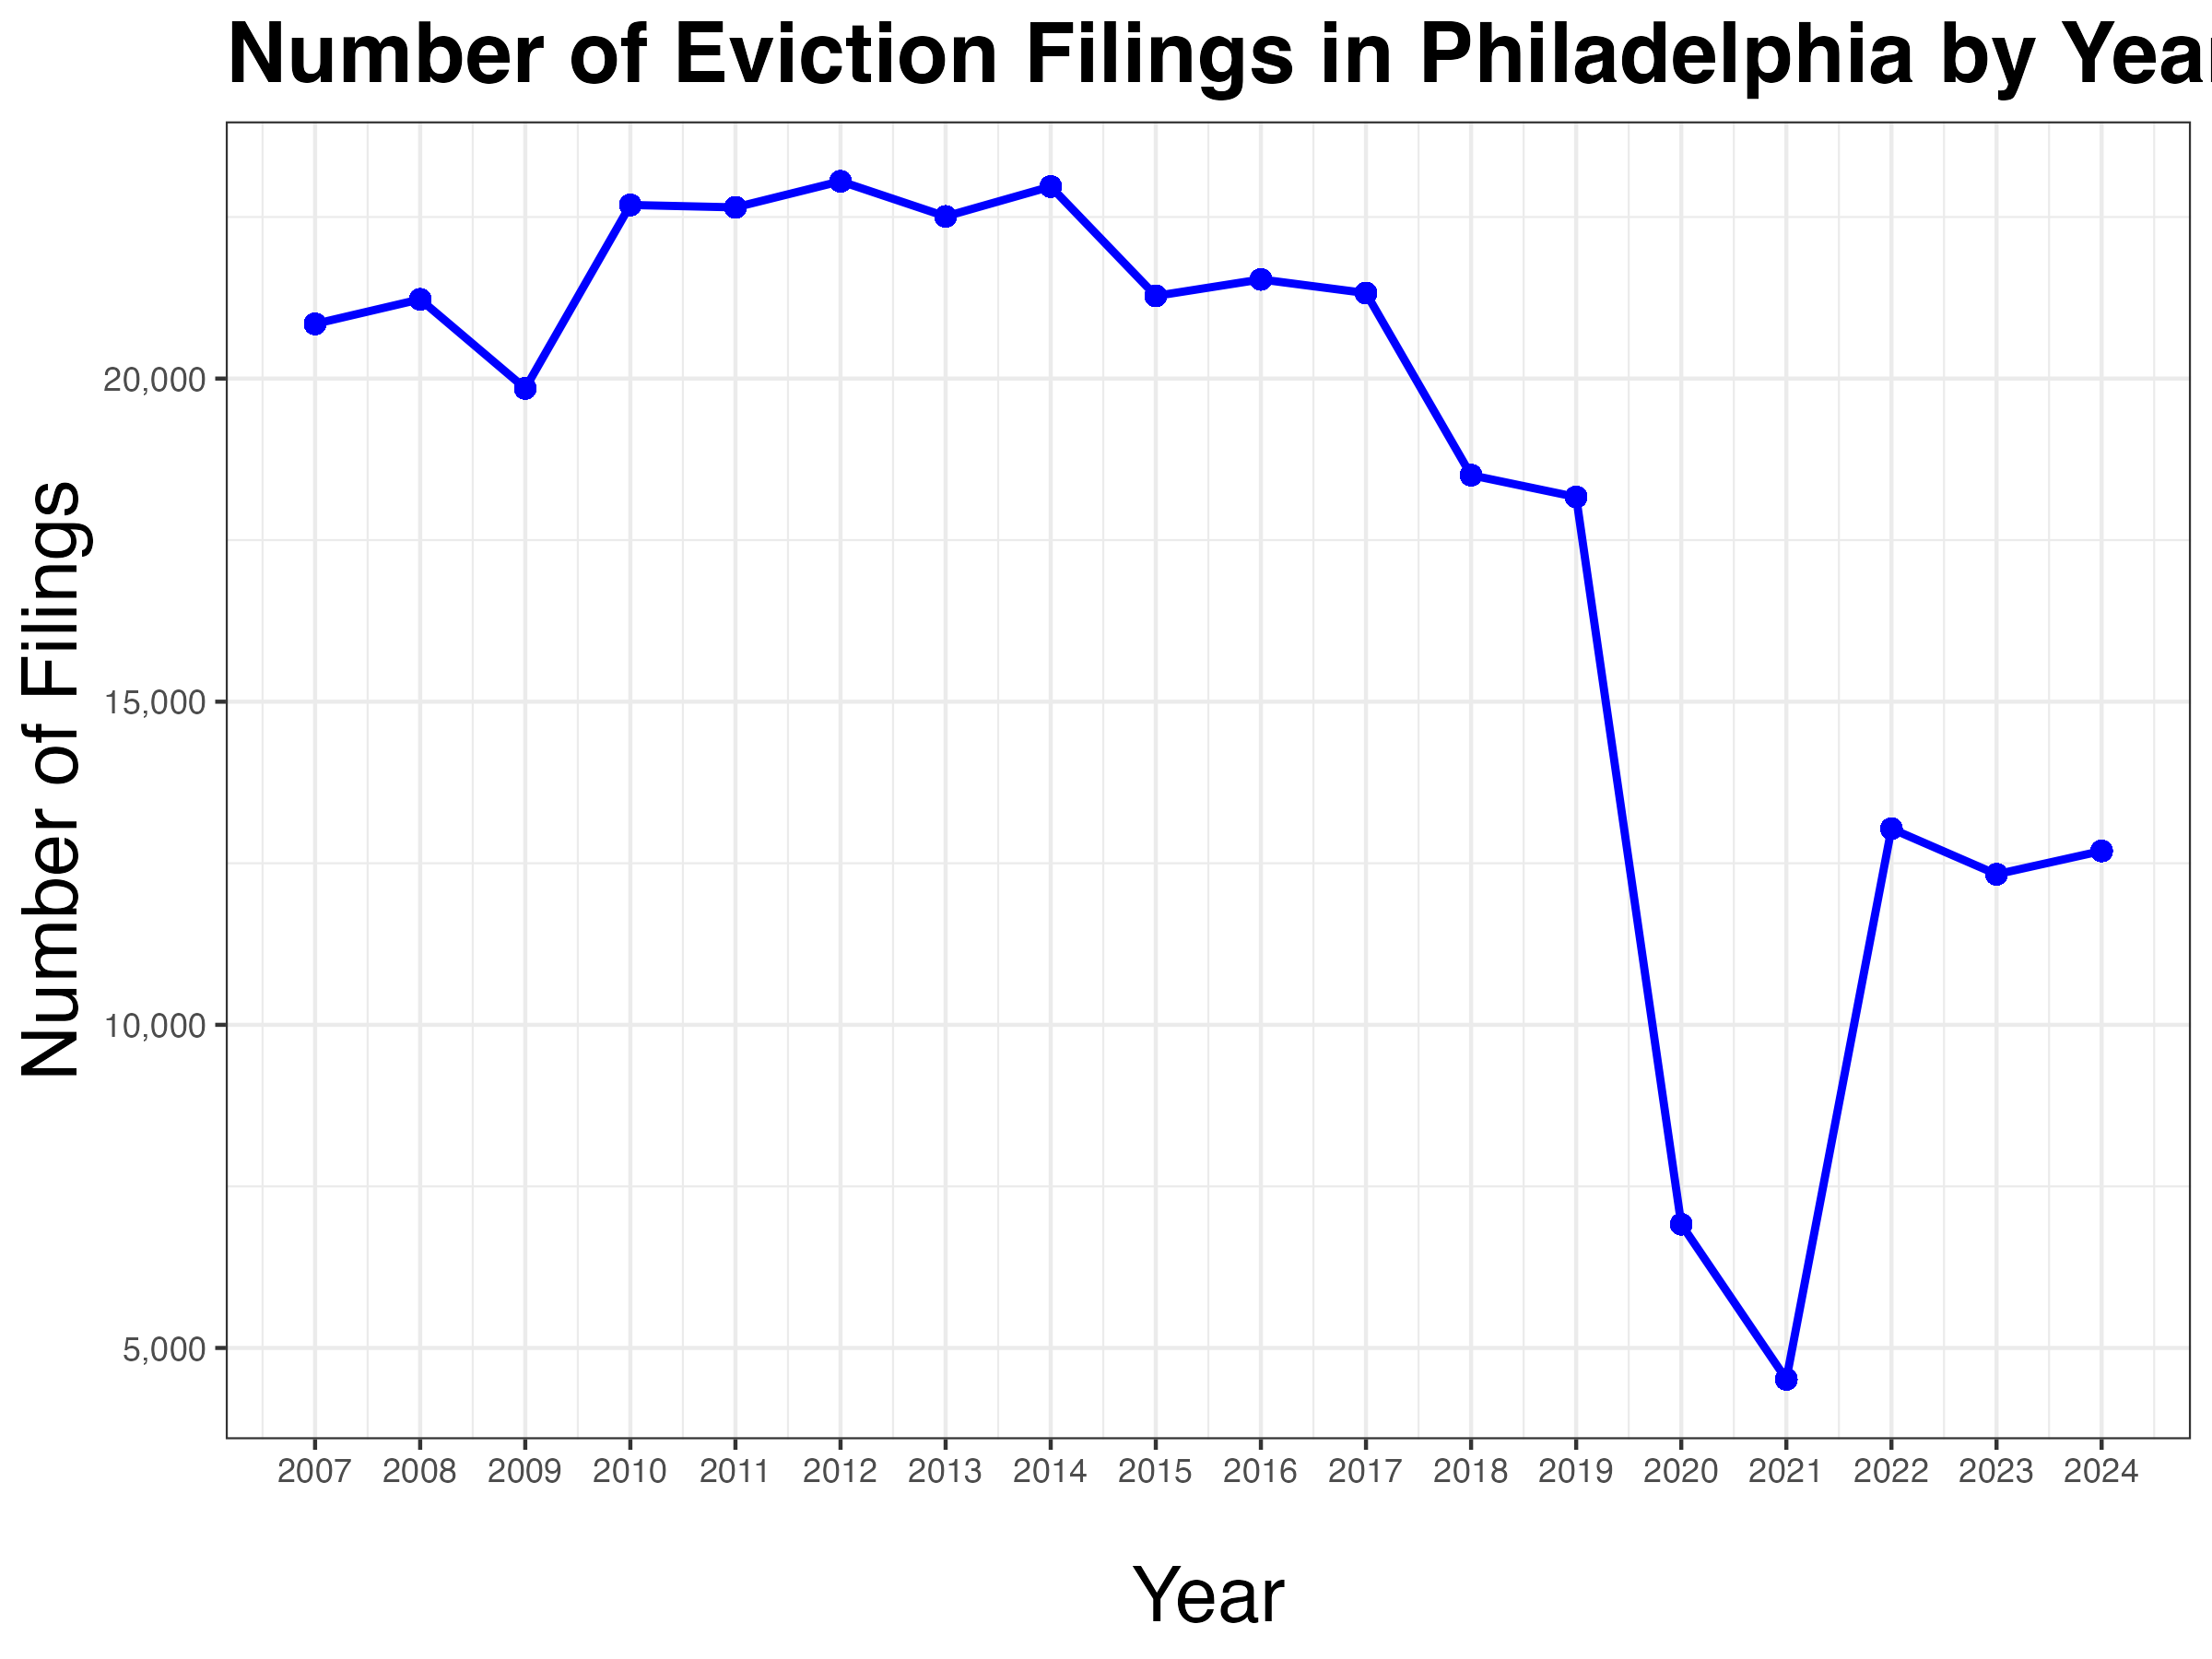
\includegraphics[width=0.75\linewidth]{figs/num_eviction_filings_by_year.png}
        \caption{Eviction Filings by Year}
        \label{fig:evict-year}
    \end{figure}
\end{frame}

\begin{frame}{Changes in landlord response by unit size}
    \begin{figure}
        \centering
        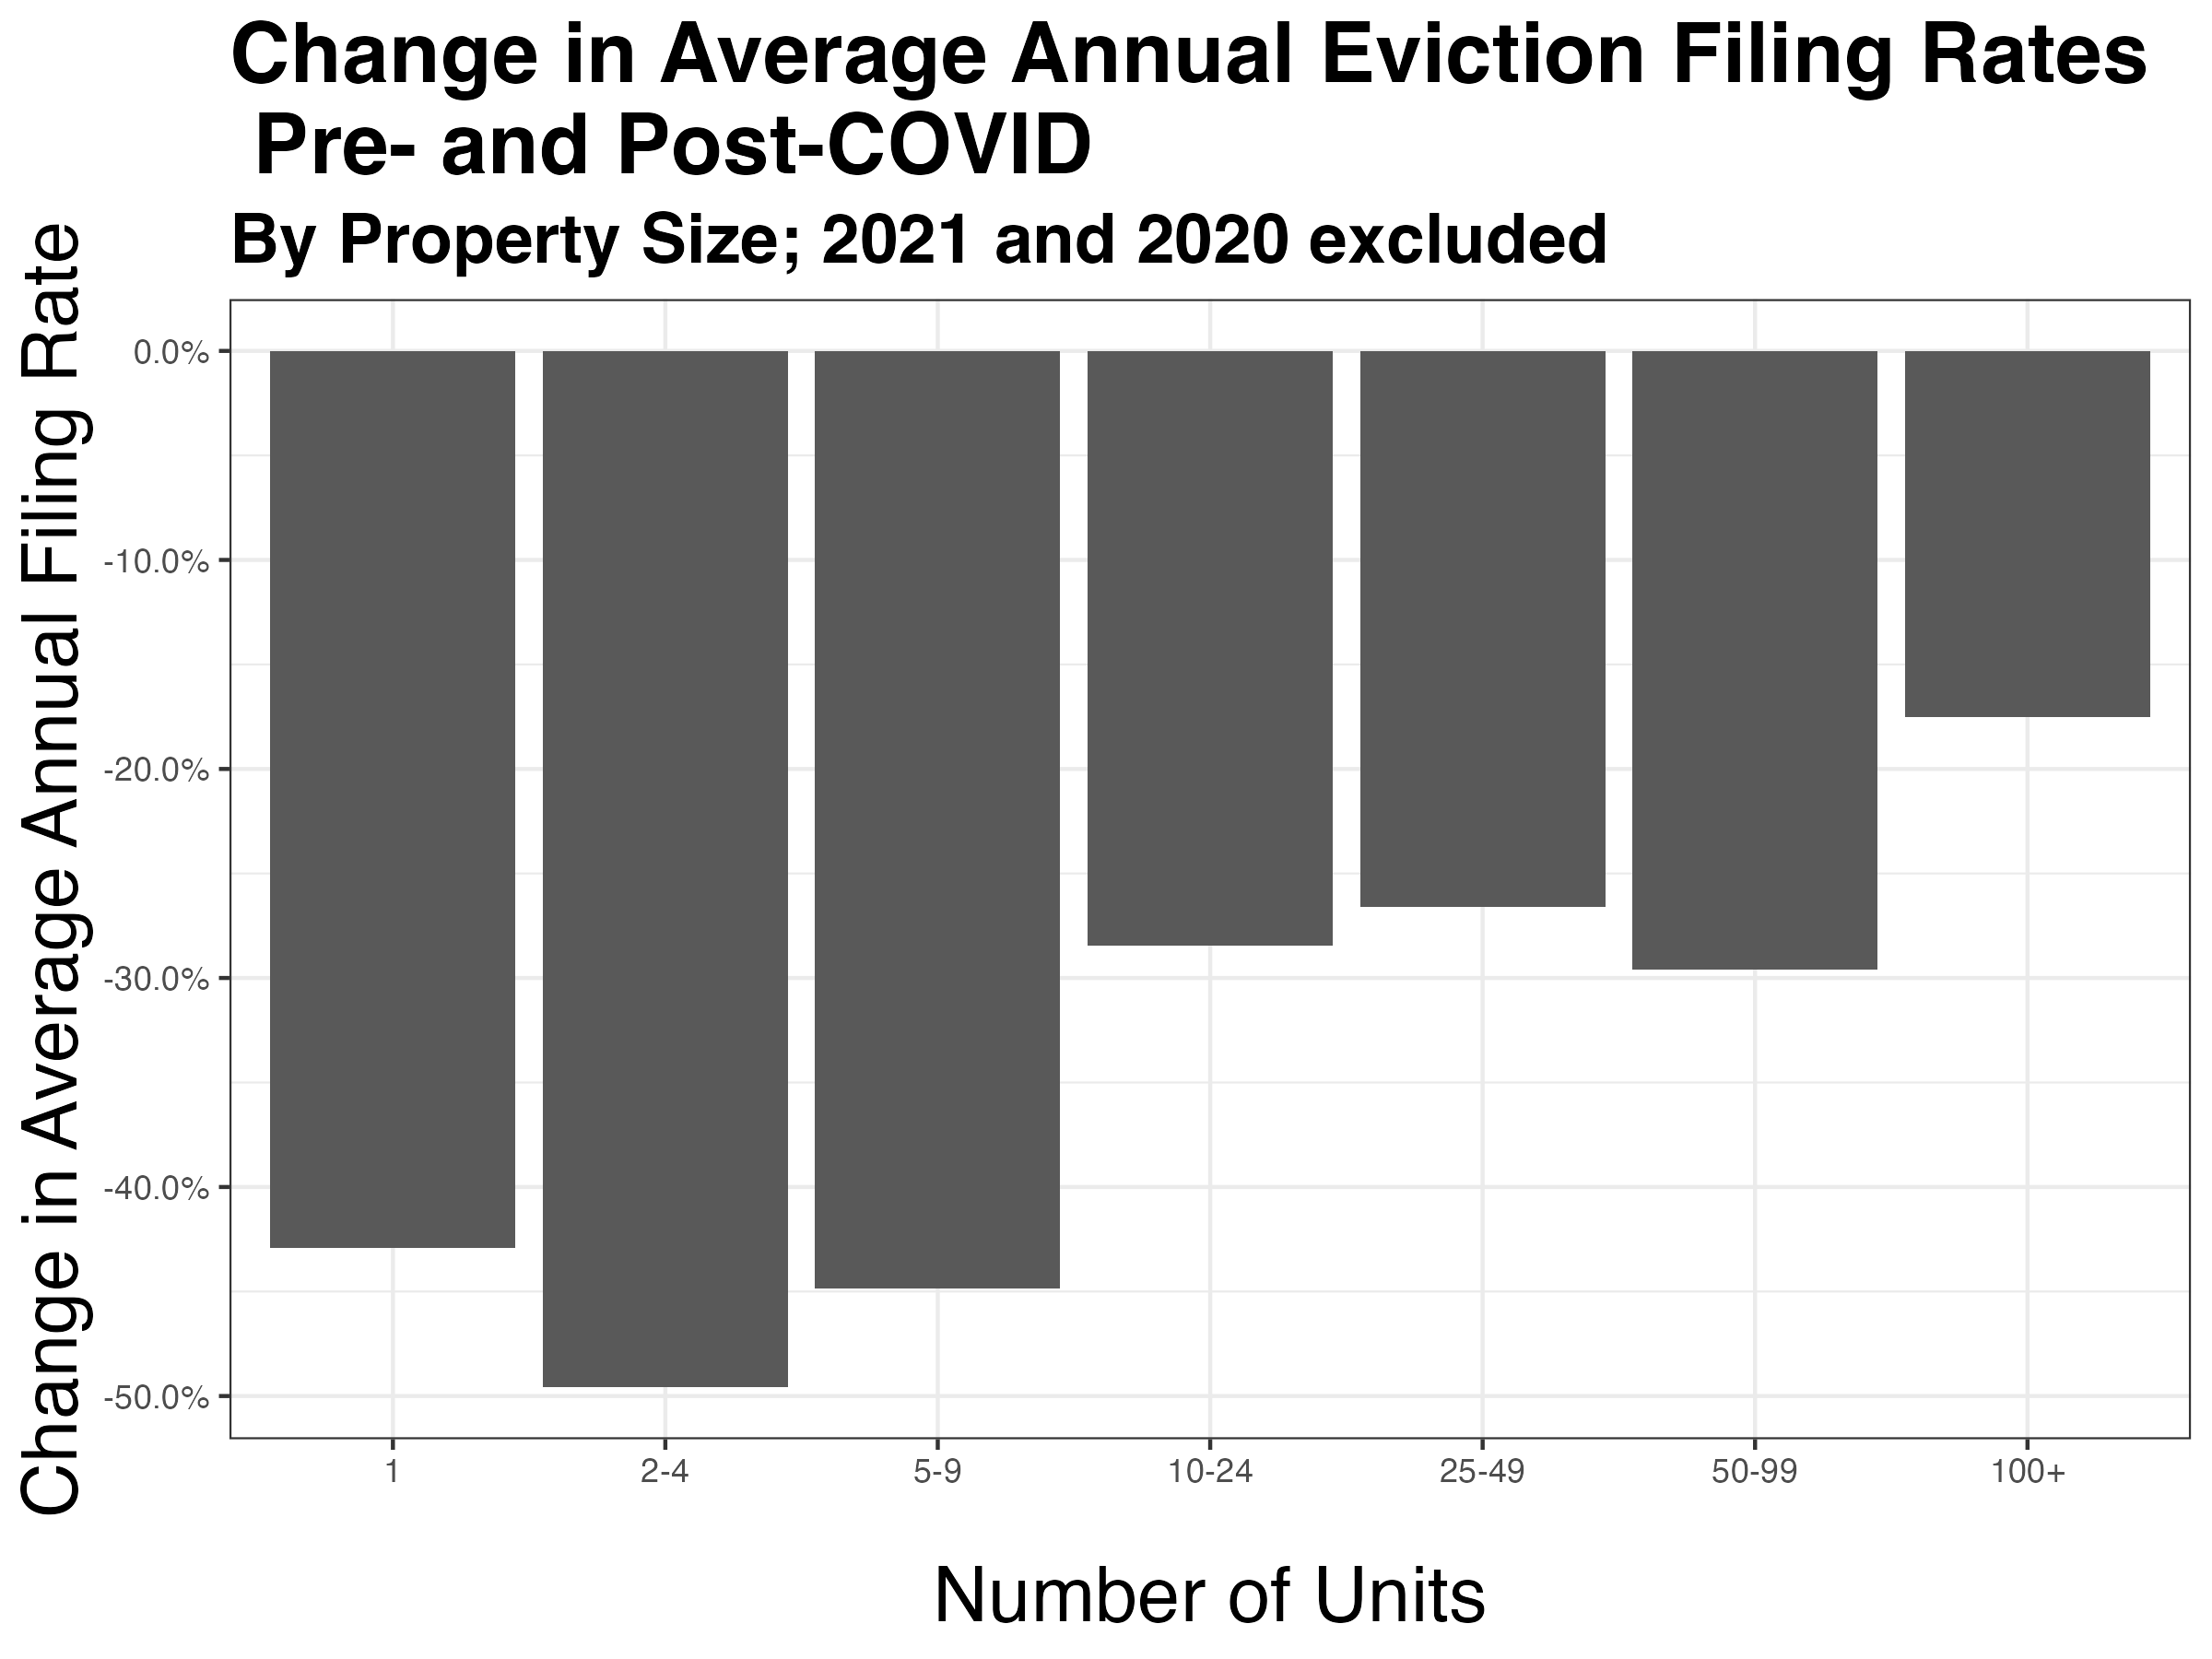
\includegraphics[width=0.75\linewidth]{figs/change_in_avg_annual_eviction_filing_rates_pre_post_COVID_by_num_units.png}
        \caption{Change in filing behavior by number of units}
        \label{fig:change-evict-units}
    \end{figure}
\end{frame}

% \begin{frame}{Evidence of Price Effects}
%     \begin{figure}
%         \centering
%         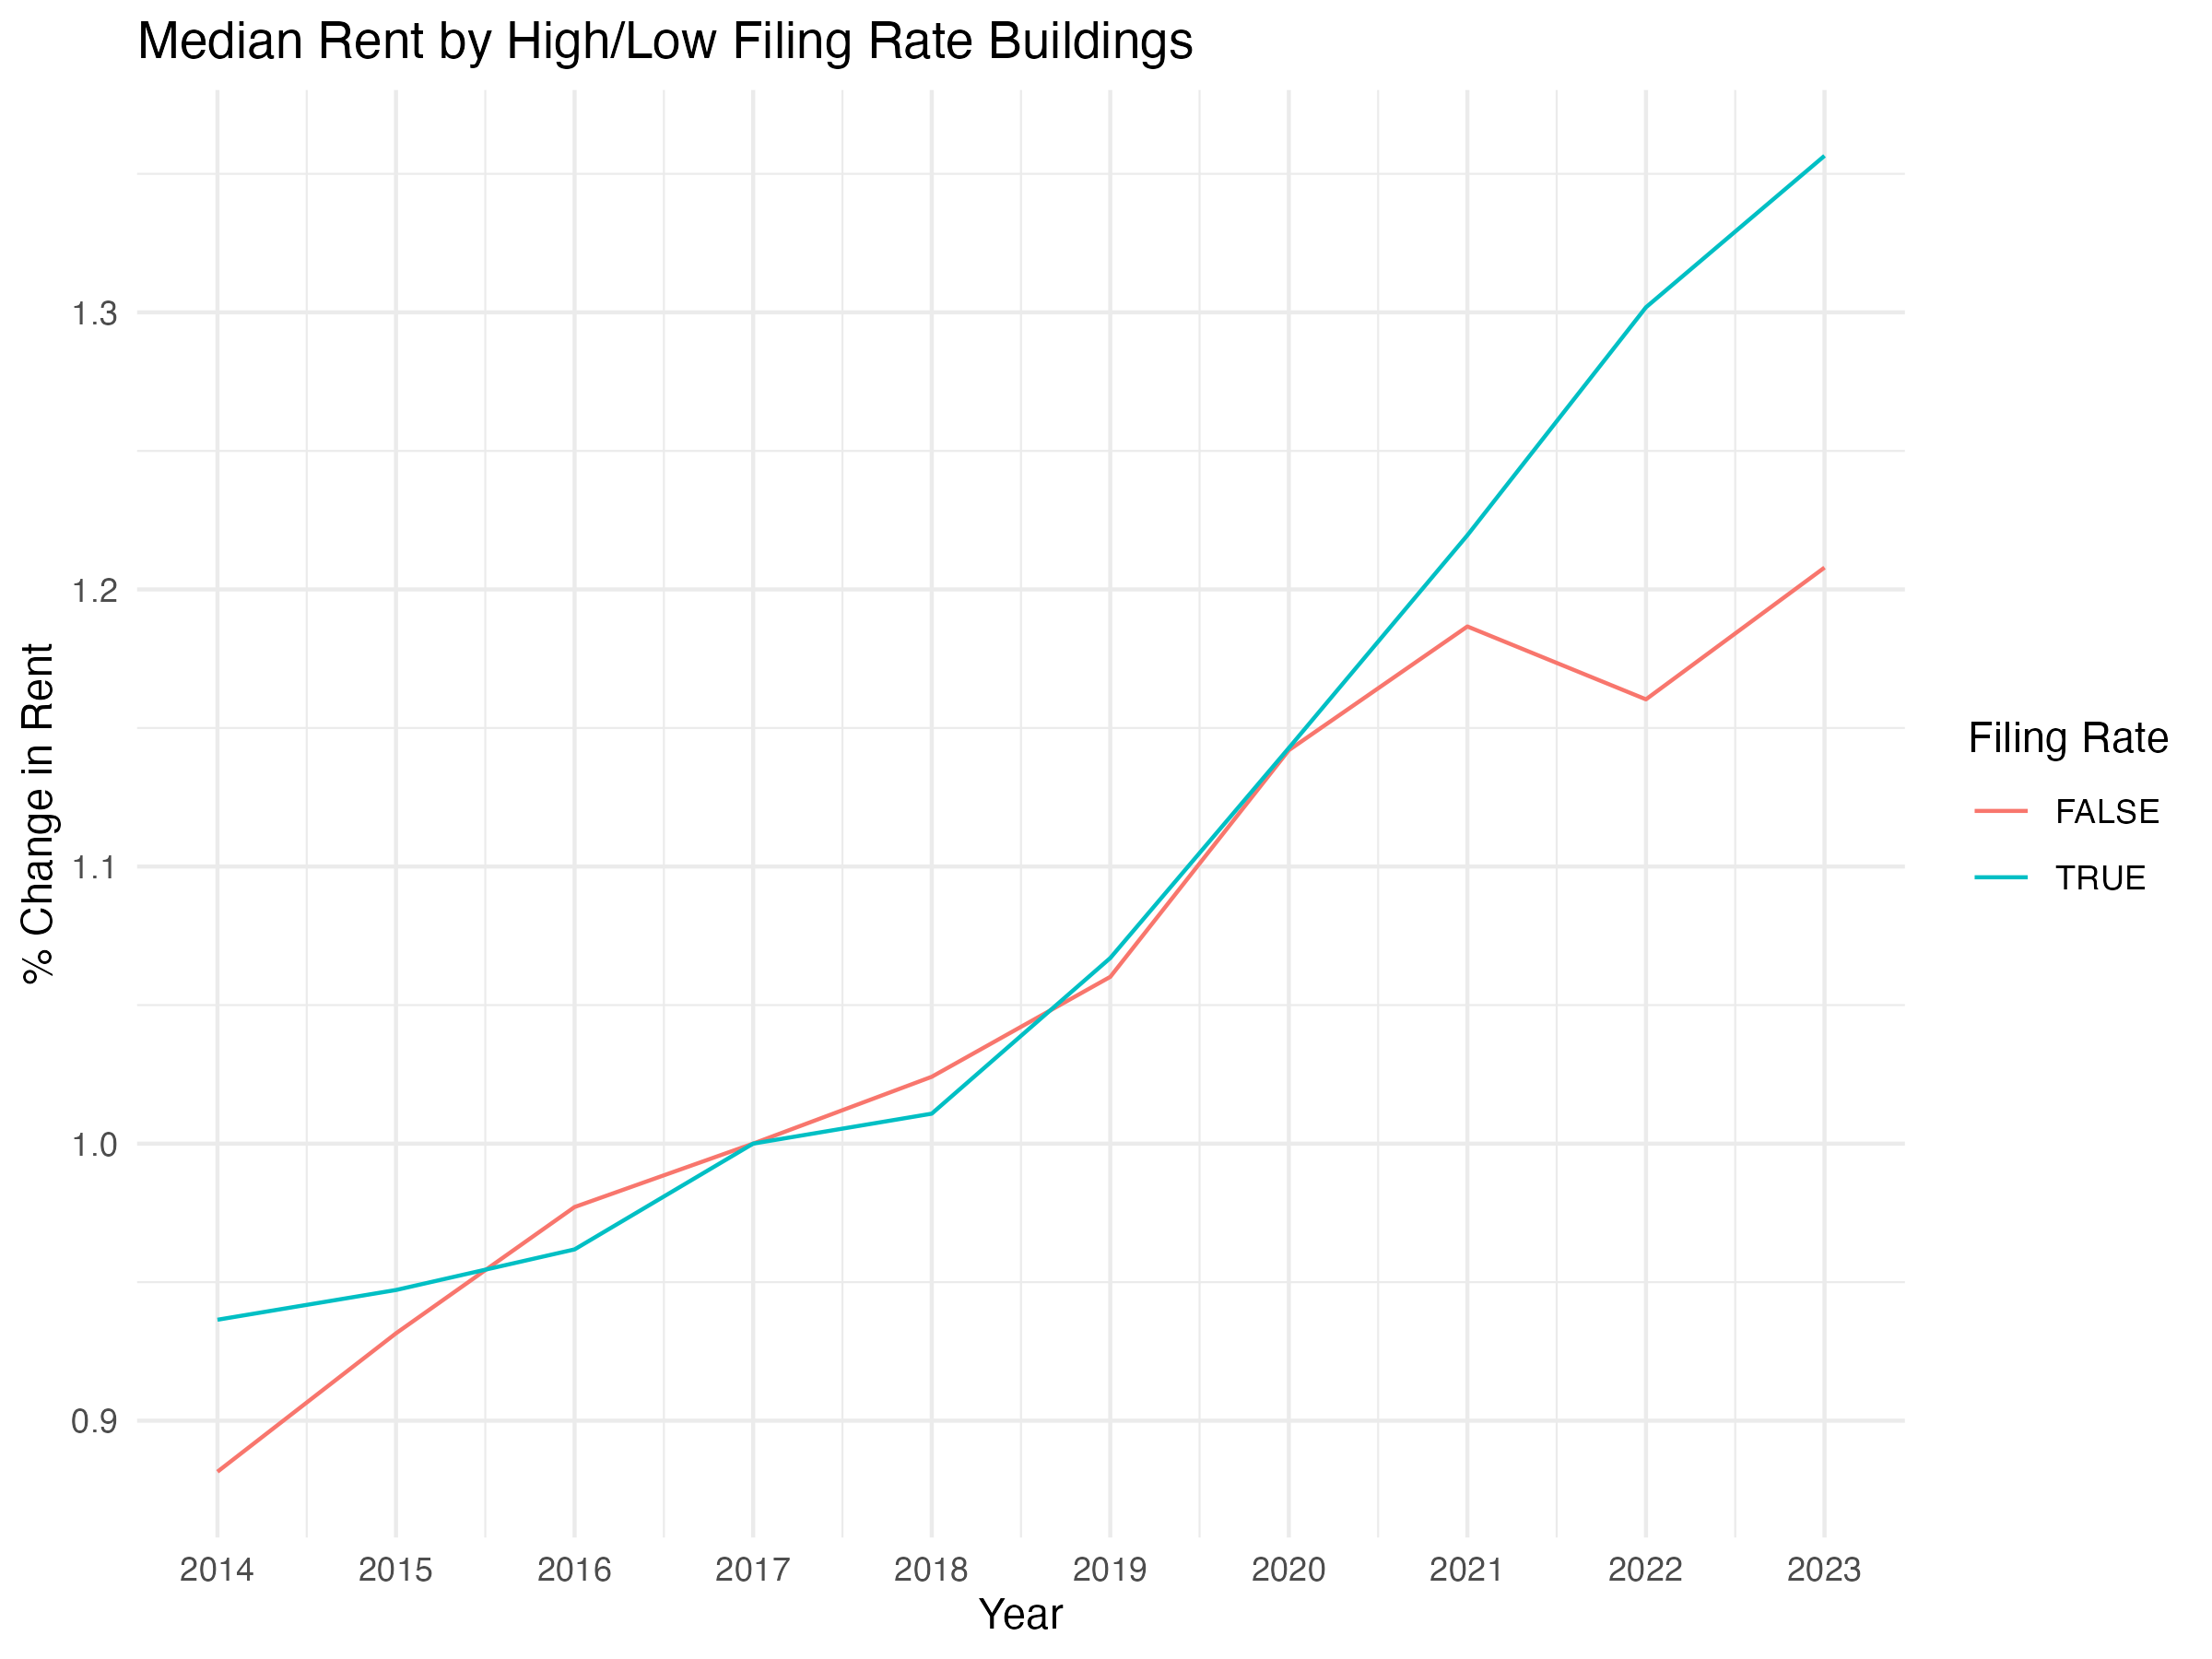
\includegraphics[width=0.75\linewidth]{figs/mean_price_quintile.png}
%         \caption{Price Changes over Time}
%         \label{fig:price-high-filing}
%     \end{figure}
    
% \end{frame}

\begin{frame}{Evidence of Price Effects}
    Here, I run an event study comparing prices of buildings with a $>10\%$ filing rate per year; there's no "treatment", so you should think of it as a price index.
    \small
    \begin{figure}
        \centering
        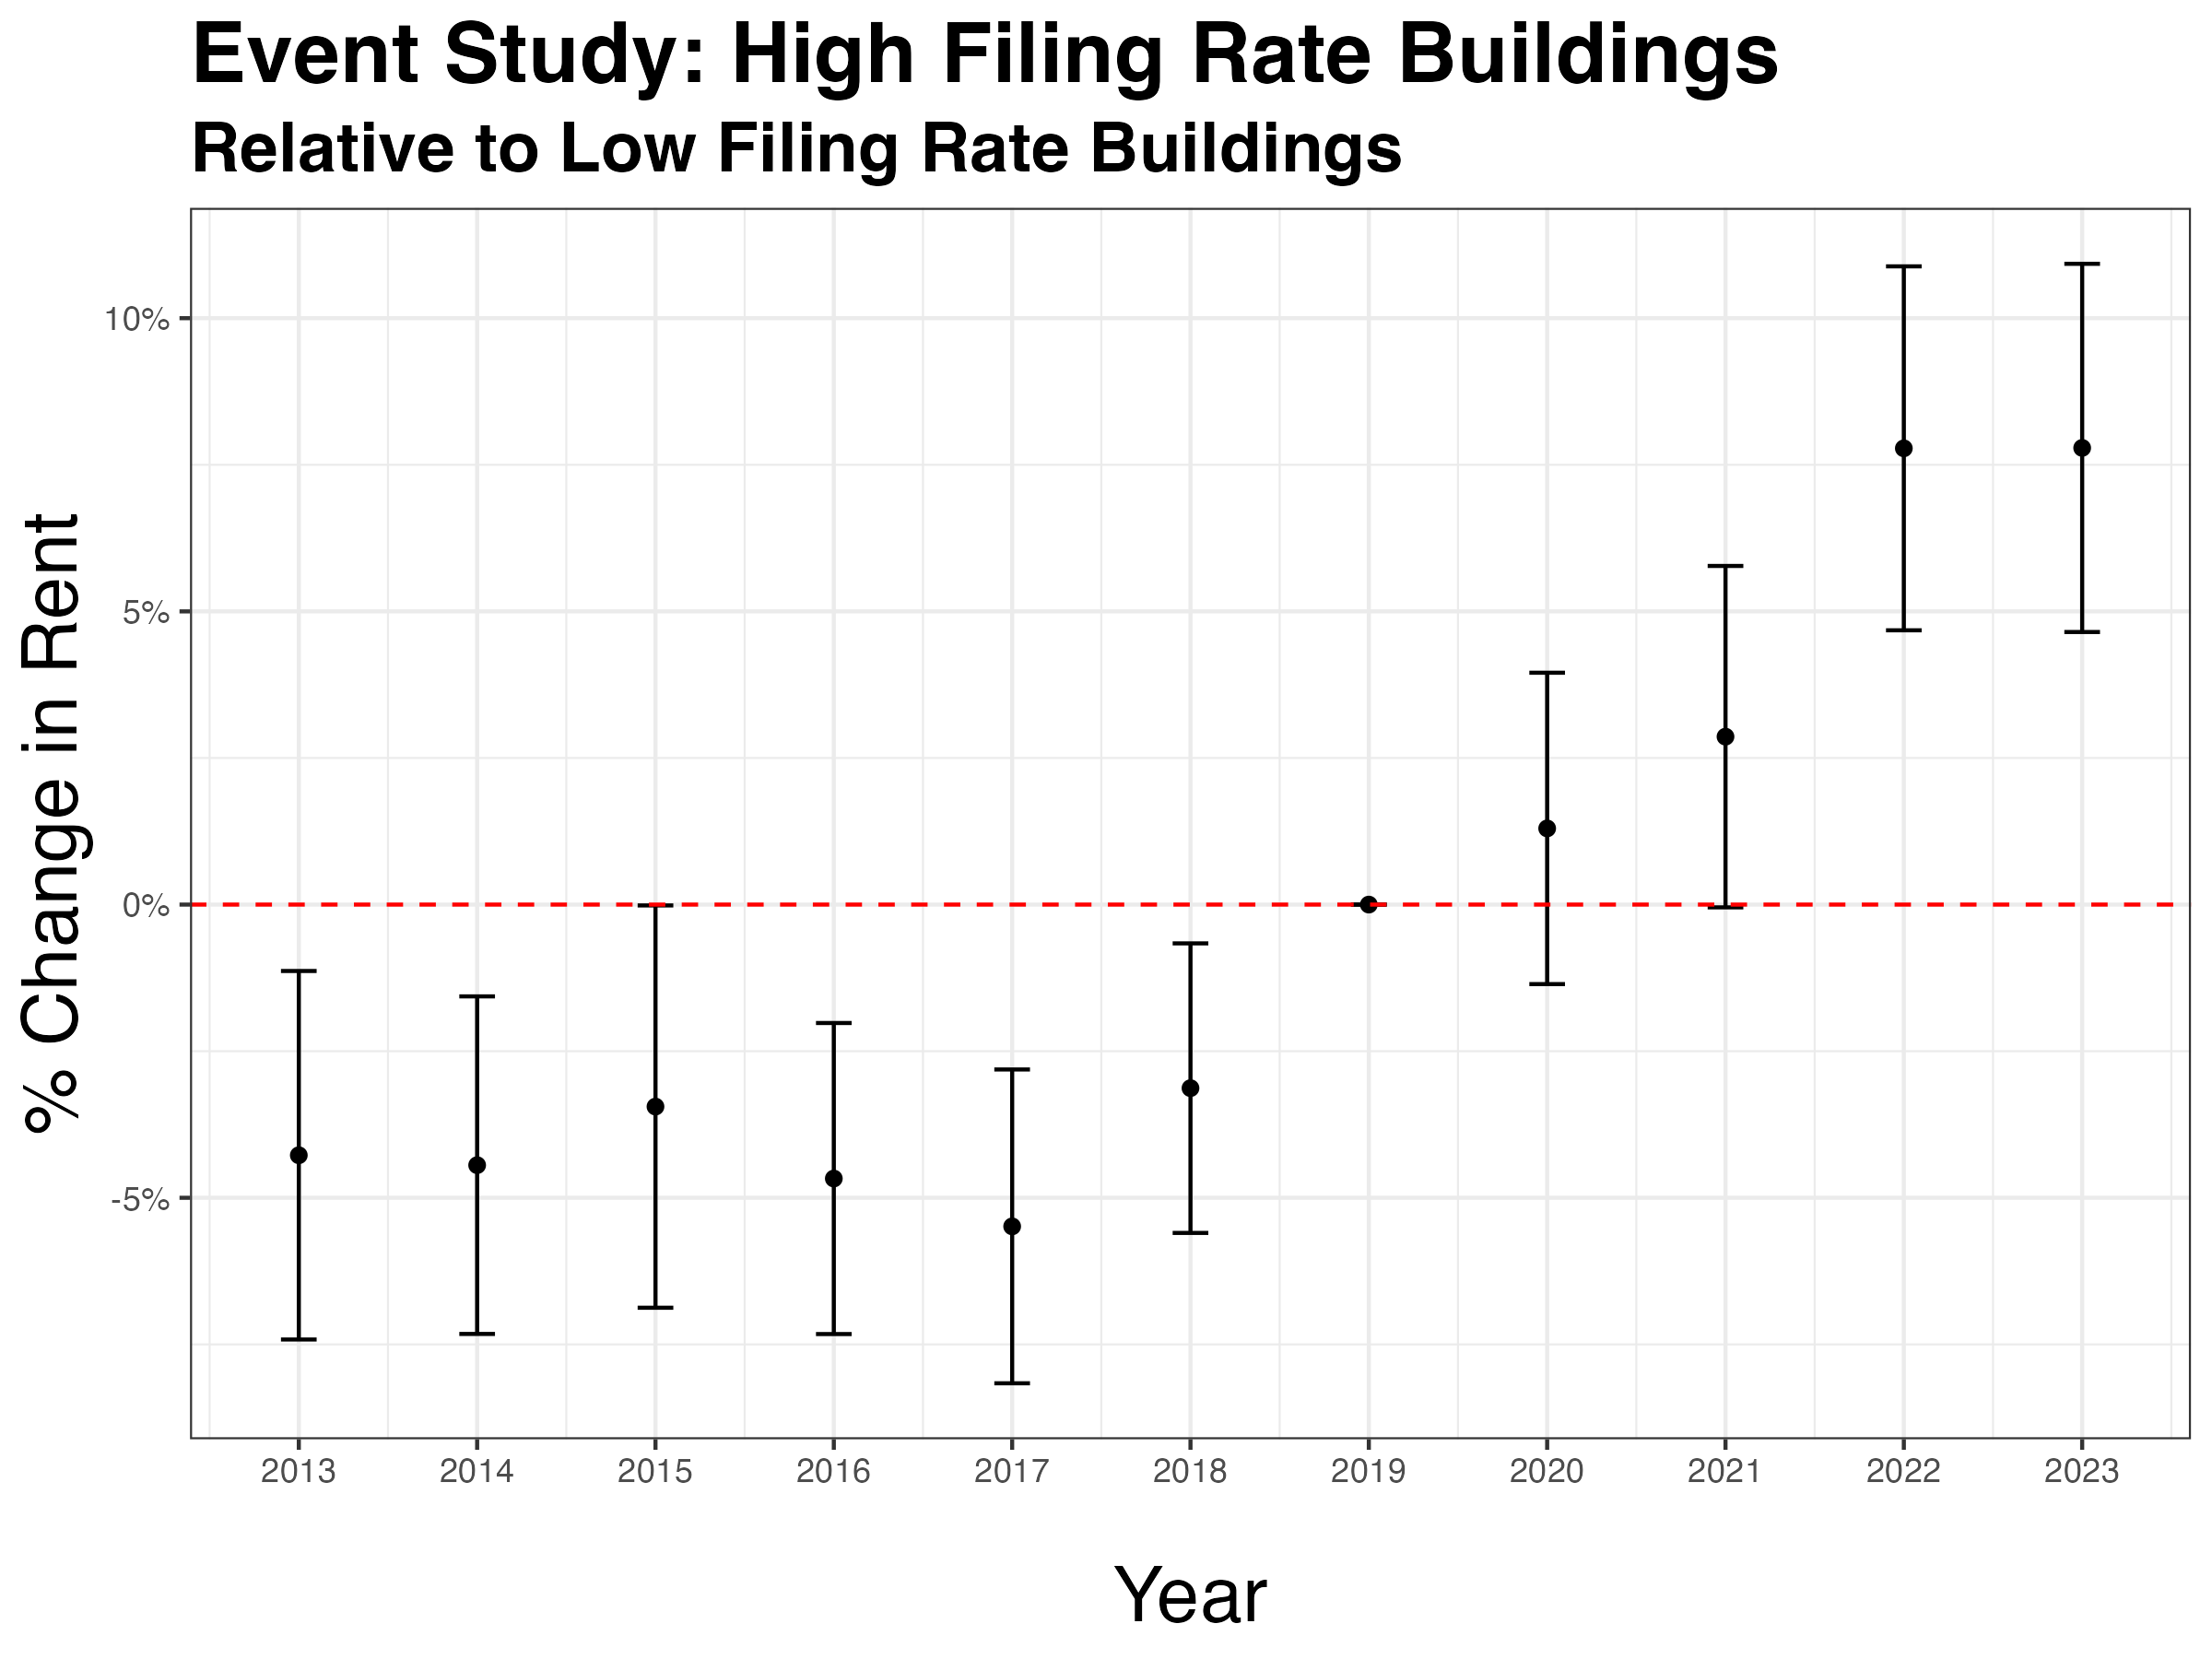
\includegraphics[width=0.65\linewidth]{figs/event_study_high_filing_preCOVID.png}
        \caption{Event Study Results}
        \label{fig:placeholder}
    \end{figure}
    
\end{frame}

\begin{frame}{Evidence of Price Effects}
    I repeat by previous price index, but I allow for census tract by year trends.
    \small
    \begin{figure}
        \centering
        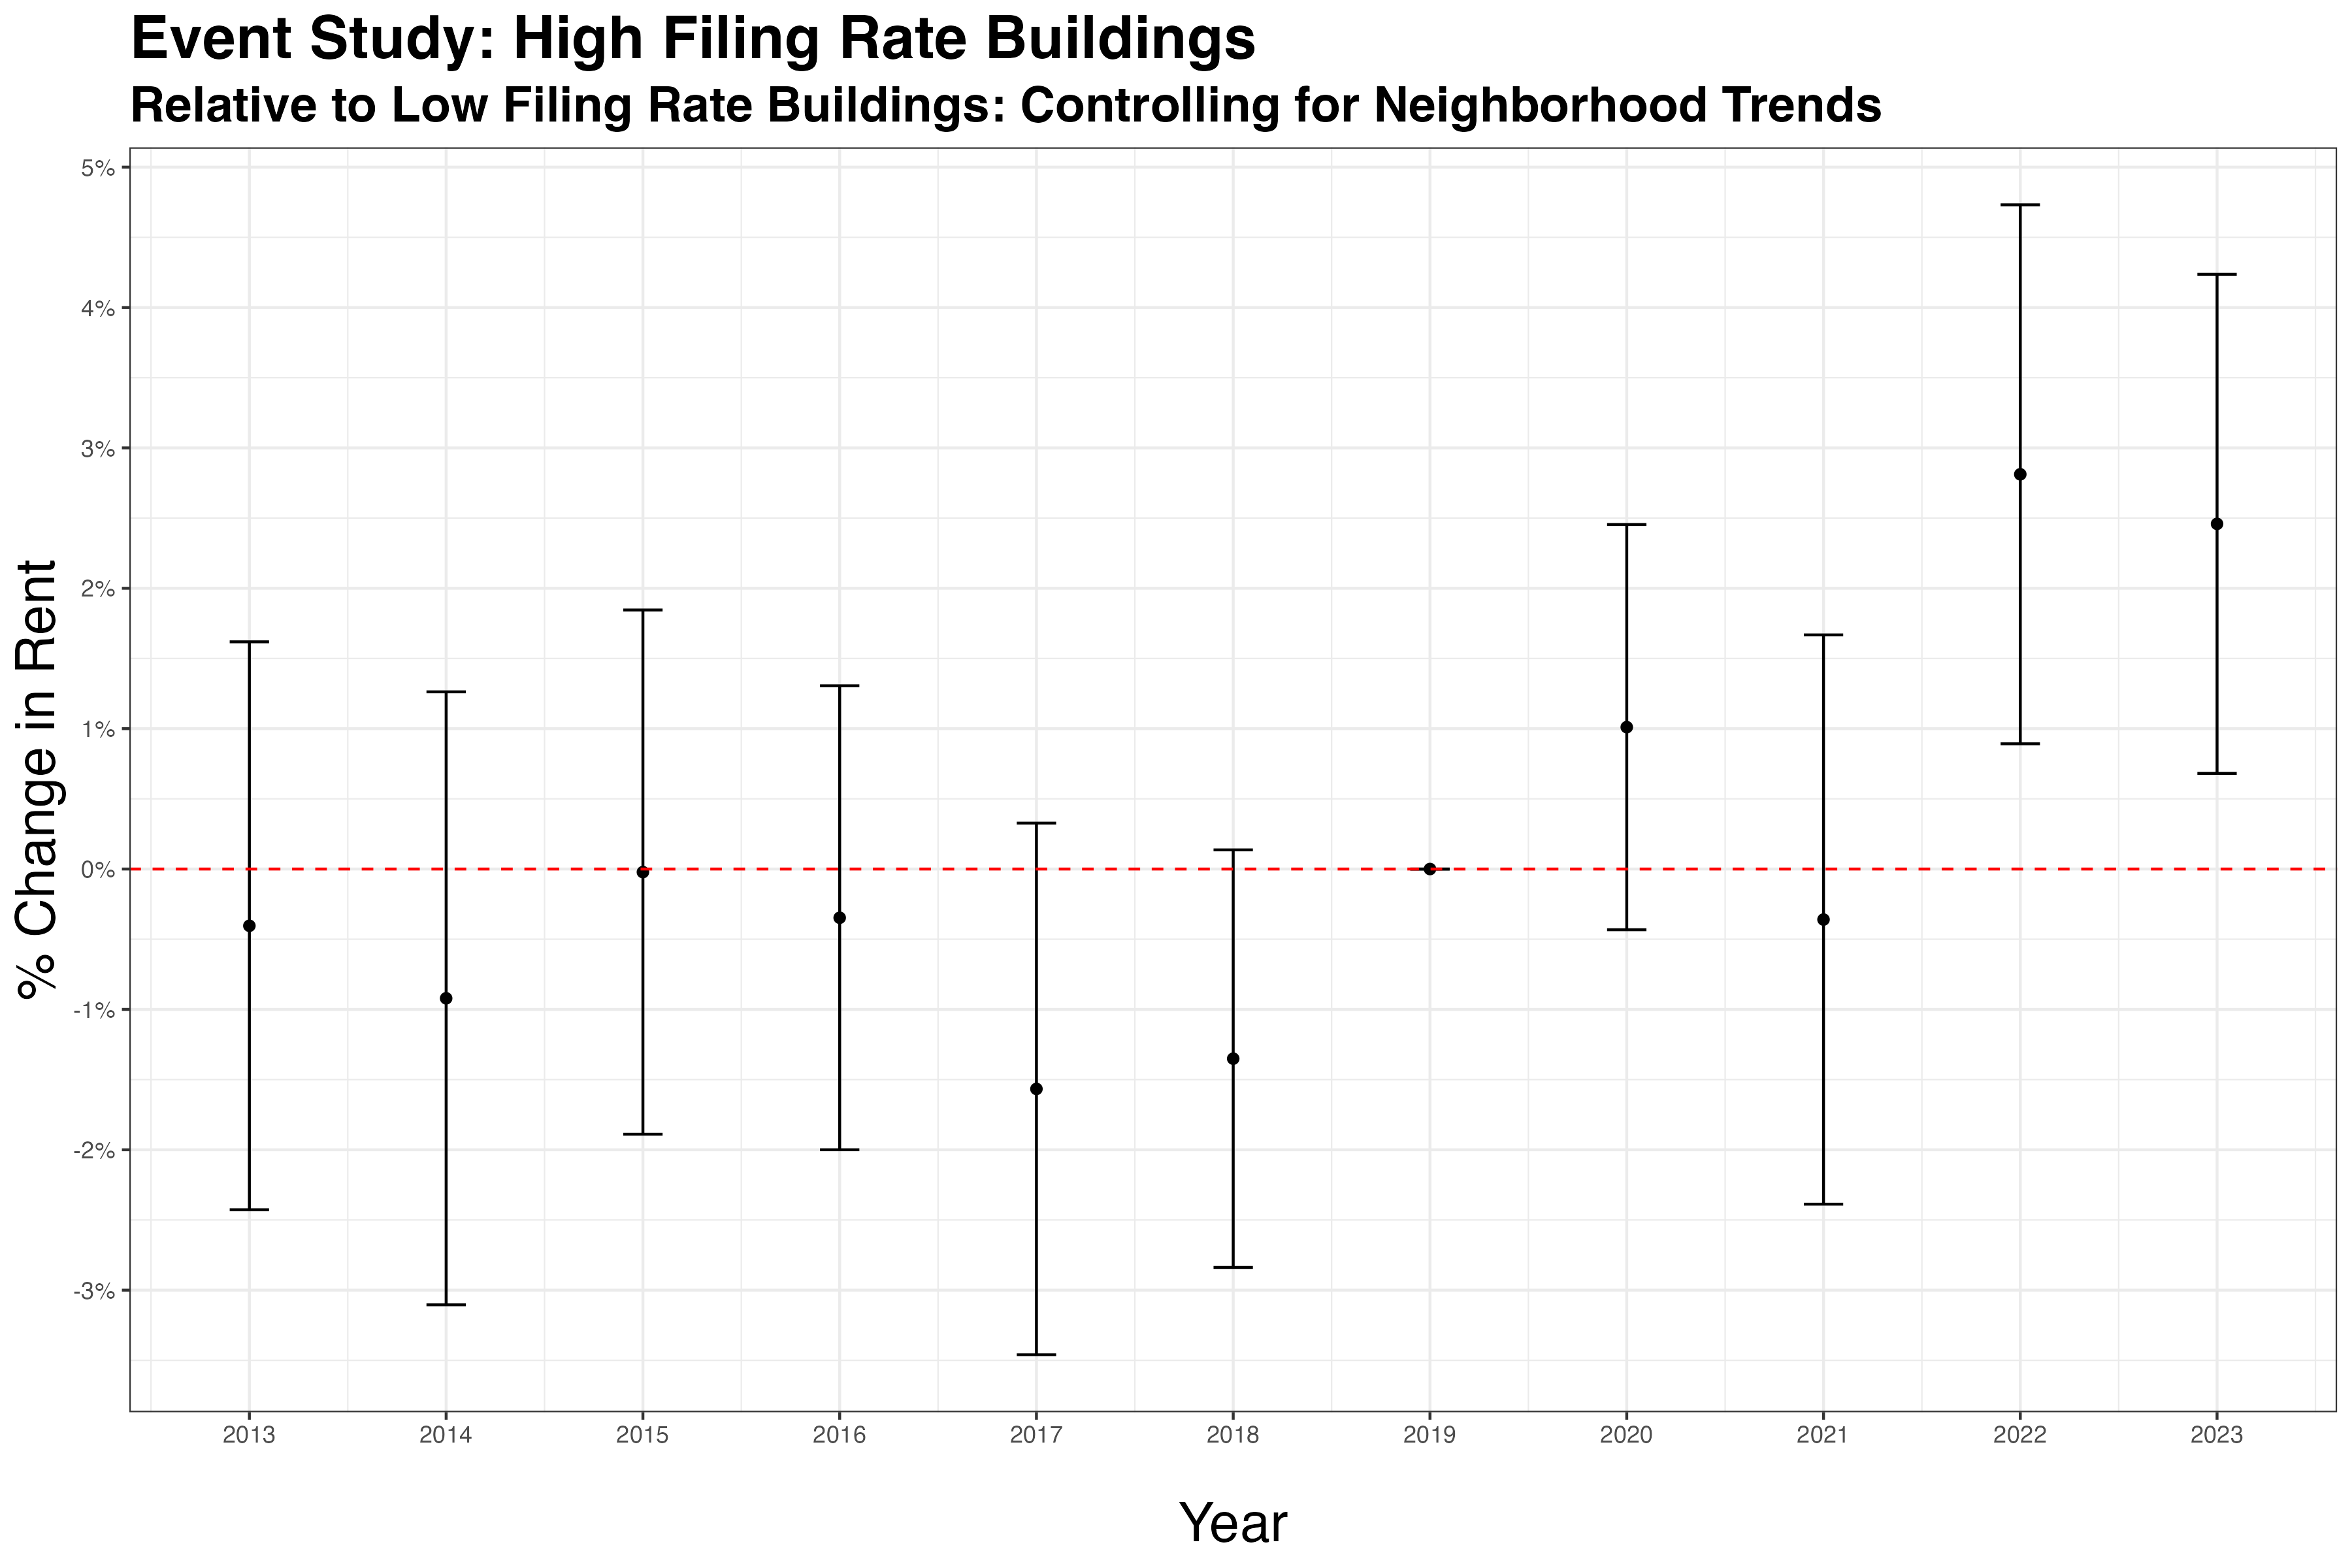
\includegraphics[width=0.65\linewidth]{figs/event_study_high_filing_preCOVID_m2.png}
        \caption{Event Study Results: Neighborhood Trends}
        \label{fig:placeholder}
    \end{figure}
    
\end{frame}


\begin{frame}{High Level Motivation of Model}
\begin{itemize}
    \item Goal is to change landlord conduct (reduce evictions) while inducing minimal pass-through onto rents
    \item The key will be that certain landlords will be closer/farther away from exit/quality upgrading/deferred maintenance 
    \item Papers in the literature \cite{diamond-2019, collinson2024eviction, } all rely on an exit mechanism to move prices; I follow their lead
    \begin{itemize}
        \item Exit ≈ quality upgrading (condo conversion), so policy effects propagate via reallocation across quality tiers
    \end{itemize}
\end{itemize}
    
\end{frame}

\begin{frame}{Toy Model Intuition}
    If the mechanism is exit, the probability of exit will depend on how good the landlord's outside option is relative to how high the cost shock was:

    \begin{figure}[t]
          \centering
          \begin{subfigure}{0.48\textwidth}
            \includegraphics[width=\linewidth]{img1}
            \caption{Philadelphia}\label{fig:left}
          \end{subfigure}\hfill
          \begin{subfigure}{0.48\textwidth}
            \includegraphics[width=\linewidth]{figs/}
            \caption{San Francisco}\label{fig:right}
          \end{subfigure}
          \caption{Two images side by side.}\label{fig:pair}
\end{figure}
    
\end{frame}


% \begin{frame}{Variation in landlord exit opportunities}
%     - put a picture of two high evicting properties
% \end{frame}


%\begin{frame}{Toy Model}

% \textbf{Model Primitives}
% \begin{itemize}
%     \item Discount rate $\delta \in (0,1]$
%     \item Exogenous initial continuum of landlords $i \in [0,1]$ that each produce one unit of housing
%     \item Inverse market demand in Period 2: $P(Q); P'(.) < 0$
%     \item Landlord profits = $P(Q) - c_i$
% \end{itemize}

% \textbf{Timing and Environment}
% Two period model. Cost shock happens between time 1 and 2.
% \begin{itemize}
%     \item At t=1, landlord draws a cost $c_i>0$ and a scrap value $s_i>0$ from a joint CDF $F(c,s)$ with correlation = $\rho$
%     \item if the landlord exits at t=1, they get the scrap value $s_i$ immediately; if they stay, they get flow profit = $P(Q) - c_i$
% \end{itemize}


% \end{frame}

% \begin{frame}{Toy Model Continued}
% \textbf{Landlord Problem}
% Landlord stays in the market iff
% \begin{align*}
%     \delta(P(Q) - c_i) \geq s_i
% \end{align*}

% Define S(p) as the set of all prices such that a landlord continues for a given $c,s$
% \begin{align*}
%     S(p) & = \big\{(c,s): c \leq p, s \leq \delta(p - c)
% \end{align*}

% Then supply is equal to 
% \begin{align*}
%     S(P) =  \int\int_{S(P)}dF(c,s)
% \end{align*}

% Markets clear such that $p*$ solves $D(p*) = S(p*)$


    
% \end{frame}

% \begin{frame}{Toy Model Comparative Statics}
% For a given price, a higher $\rho$ shifts out the set of landlords who will exit, so $S(P)$ increases with $\rho$. Since demand slopes downwards, this means $\frac{dp*}{d\rho} >0$\\

% Intuitively, price response will be worse in a world where more marginal landlords are targeted by the cost increase
    
% \end{frame}

% \begin{frame}{Toy Model Continued}
%     In reality, landlords have more options than a simple exit/continue decision:
%     - change screening practices
%     - quality upgrading
%     - immediate exit
%     Covariance between adjustment mechanisms and cost increases will be determinant of price hike. Degree of market segmentation will also affect price responses
% \end{frame}

\begin{frame}{Toy Model Nested Logit}
    \begin{itemize}
        \item Two period model with discount rate $\delta =1$
        \item Exogenous initial continuum of landlords $i \in [0,1]$ that each produce one unit of housing
        \item Low nest ($L$) and high nest ($H$); each landlord is active in one nest
        \item Market size $M$ is exogenous and normalized to $J=n_l +n_h$
        \item At t=1, \textbf{low tier landlords} draw costs $\kappa_i>0$, and a quality upgrading cost $\phi_i>0$ from a joint CDF $F(\kappa,\phi)$ with correlation = $\rho$
        \item \textbf{low tier landlords} can now pay an upgrade cost $\phi_i$ to enter the high tier (and avoid paying $\kappa_i$), or continue and make low tier flow profits
        \begin{itemize}
            \item Normalize marginal cost = 0, so $\pi_g=p_g$
        \end{itemize}
    \end{itemize}    
\end{frame}

\begin{frame}{Toy Model Cont.}
    Product $j$ in nest $g(j)$ has mean utility $\delta_j$; price coefficient $\alpha>0$; nest correlation (segmentation) $\sigma\in[0,1)$. \\
    
    Within-nest shares and inclusive values:
        \begin{align*}
            s_{j|g} \;=\;
            \frac{\exp\!\left(\frac{\delta_j-\alpha p_j}{1-\sigma}\right)}
            {\sum_{k\in g}\exp\!\left(\frac{\delta_k-\alpha p_k}{1-\sigma}\right)},
            \qquad
            I_g \;=\; (1-\sigma)\,\log\!\sum_{k\in g}\exp\!\left(\frac{\delta_k-\alpha p_k}{1-\sigma}\right).
        \end{align*}
    Nest shares (no outside):
        \begin{align*}
            S_g \;=\;\frac{e^{I_g}}{e^{I_L}+e^{I_H}},
            \qquad
            s_j \;=\; S_{g(j)}\,s_{j|g(j)},
            \qquad
            S_L+S_H \;=\; 1.
        \end{align*}
    
    Assuming products are homogenous within a nest: 
        \begin{align*}
            \boxed{\,s_j=\tfrac{1}{J},\;\; s_{j|g}=\tfrac{1}{n_g},\;\; S_g=\tfrac{n_g}{J}\,}.
        \end{align*}
    
\end{frame}

\begin{frame}{Nested Logit Pricing}
    With symmetry in nest $g$, the optimal \emph{per-product markup} is
        \begin{align*}
            p_g \;=\; \frac{s_j}{\alpha\big[1 - \sigma(1-s_{j|g}) - (1-\sigma)(1-S_g)\big]}.
        \end{align*}
plugging the symmetric shares $s_j=\tfrac{1}{J}$, $s_{j|g}=\tfrac{1}{n_g}$, $S_g=\tfrac{n_g}{J}$:
\begin{align*}
\boxed{
\,p_g 
\;=\;
\frac{1}{\alpha\,J\Big(1 - \sigma\!\big(1-\tfrac{1}{n_g}\big) - (1-\sigma)\!\big(1-\tfrac{n_g}{J}\big)\Big)}\;,\quad g\in\{L,H\}.
}
\end{align*}
Because $M=J$ and $s_j=1/J$, each seller’s quantity is $1$, so \emph{per-seller operating profit equals the markup}:
\begin{align*}
    \boxed{\,\Pi_g(n_L,n_H) \;=\; p_g \,}.
\end{align*}
    
\end{frame}

\begin{frame}{Nested Logit Comparative Statics}
    \textbf{Landlord choice (upgrade vs stay in L) with $(\kappa_i,\phi_i)$ correlated.}
Given a draw $(\kappa_i,\phi_i)$:
\begin{align*}
\pi_i^{L} &= p_L - \kappa_i, 
&
\pi_i^{H} &= p_H-\phi_i.
\end{align*}

%For simplicity, assume $\pi_h = \pi_l$
Then the landlord upgrades iff $\kappa_i \geq \phi_i + (\pi_h - \pi_l)$\\
Define the set of landlords that upgrade as \[
\mathcal{U}(\Delta)\;\equiv\;\big\{\, i \in \mathcal{I}\;:\; \kappa_i \geq \phi_i+ (\pi_h - \pi_l) \,\big\}
\]
\pause
Intuitively, when $\rho$ is negative, you see more exit as higher cost shocks have better outside options. \\

Further, for a given amount of exit, the price effect is higher when the rental market is more segmented.

\end{frame}

\begin{frame}{Brief Recap}
    \begin{itemize}
        \item Philadelphia's eviction overhaul seems to have worked
        \pause
        \item There's preliminary evidence of price pass-through for high evicting buildings
        \pause
        \item Toy model suggests price pass-through depends on degree of exit (which depends on landlord outside options), as well as market segmentation
        \pause
        \item For landlords that don't want to exit, I might want to build in whether they adjust on other margins
    \end{itemize}
    
\end{frame}

\section{Evidence of Market Segmentation}

\begin{frame}{Evidence of Market Segmentation}
    Infutor data let me track households as they move. Intuitively, if people at high evicting properties are more likely to move to high evicting properties, this is evidence of market segmentation. Formally, I regress:

    \begin{align*}
        FilingRate_{destination} = &\beta_0 +\mathbf{\beta_1FilingRate_{origin}} + \\&\beta_2OriginControls + \beta_3DestinationControls 
    \end{align*}
    where Origin/Destination controls will include census tract fixed effects, property size fixed effects, and log(rent)
\end{frame}

\begin{frame}{Evidence of Market Segmentation: Cont.}
    \tiny
    \begin{table}[htbp]
   \caption{\label{tab:evict_persist} Effect of Previous Eviction Filing Rate on Current Filing Rate}
   \centering
   \begin{tabular}{lccc}
      \tabularnewline \midrule \midrule
      Dependent Variable: & \multicolumn{3}{c}{filing\_rate}\\
      Model:                        & (1)            & (2)            & (3)\\  
      \midrule
      \emph{Variables}\\
      Previous Eviction Filing Rate & 0.1696$^{***}$ & 0.0701$^{***}$ & 0.0522$^{***}$\\   
                                    & (0.0051)       & (0.0055)       & (0.0151)\\   
      Rent (current)                &                &                & -0.0551$^{***}$\\   
                                    &                &                & (0.0070)\\   
      Rent (previous)               &                &                & 0.0021\\   
                                    &                &                & (0.0047)\\   
      \midrule
      \emph{Fixed-effects}\\
      Units (current)               &                & Yes            & Yes\\  
      Units (previous)              &                & Yes            & Yes\\  
      Census Tract (current)        &                & Yes            & Yes\\  
      Census Tract (previous)       &                & Yes            & Yes\\  
      \midrule
      \emph{Fit statistics}\\
      Observations                  & 125,685        & 88,035         & 7,998\\  
      \midrule \midrule
      \multicolumn{4}{l}{\emph{Clustered (pid) standard-errors in parentheses}}\\
      \multicolumn{4}{l}{\emph{Signif. Codes: ***: 0.01, **: 0.05, *: 0.1}}\\
   \end{tabular}
\end{table}

\end{frame}

\begin{frame}{Evidence of Market Segmentation: Nested Logit}
    \begin{itemize}
        \item Consider a renter's choice set as all the units in a zip code by building type by year (1 unit; 2-4 units, 5-50 units; 51+ units, following \cite{framoutar2024market, calderwang2024algorithmic})
        \begin{itemize}
            \item Because of issues with choice probabilities sometimes near zero, I drop buildings with fewer than 5 units
        \end{itemize}
        \pause
        \item Renters first choose a nest (n) (high / low evicting), then choose a market (j), and finally a product (i) (building) within that market
        \pause
        \item Household utility is then \begin{align}
            U_{ijt}
              &= \alpha p_{jt} + x_{jt}\beta^{\mathrm{ex}} + \xi_{jt}
                 + \bar{\epsilon}_{h(j)ti} + (1-\rho)\,\tilde{\epsilon}_{ijt} \tag{6} \\[6pt]
                 \end{align}
        \item Where $x_{jt}$ are product characteristics including log(market value),log(total area), year built, and fixed effects for quality grade, building type, and census tract by year
        \pause
        \item Outside good is renting a unit within the market, which does not appear in my data (typical outside good share is ~70\%).
    \end{itemize}
    
\end{frame}

\begin{frame}{Nested Logit Share Construction}
    \begin{itemize}
        \item In Philadelphia, the median housing unit is close to 100 years old and there is relatively little entry, especially in poorer areas
        \item Lack of recent entry necessitates using occupancy rates as a measure of quantity (and thus, shares)
        \item Solution is to use Infutor address changes to infer occupancy rates
        \begin{itemize}
            \item For full disclosure, I'm still working on sanity checking how well this works, particularly for lower income areas, where coverage is less good
        \end{itemize}
        \item Given occupancy rates, shares are defined as the number of occupied units in a building divided by the total number of occupied units in that market
    \end{itemize}
    
\end{frame}

\begin{frame}{Nested Logit Instruments}
    \begin{itemize}
        \item I instrument for $\rho$ using the number of products in the nest
        \item For this presentation, I treat price as exogeneous.
        \begin{itemize}
            \item Obviously this isn't ideal, however, the instruments I tried were all very weak, and I'll show my estimates are reasonable. If people have thoughts on the weak instruments issue, let me know!
        \end{itemize}
    \end{itemize}
    
\end{frame}

\begin{frame}{Nested Logit Results}
    \small
    \begin{table}[!htbp]
\centering
\caption{Simple Logit Estimates (N=4231, Markets=302, Products=1553; $\rho=0.682$)}
\label{tab:blp_logit_coef}
\begin{tabular}{lrrrr}
\toprule
Variable & Estimate & Std. Error & t-stat & p-value \\
\midrule
x1 & -0.1950 & 0.0403 & -4.8356 & 0.0000 \\
x2 & 0.4337 & 0.0364 & 11.9064 & 0.0000 \\
x3 & -0.0733 & 0.0222 & -3.3017 & 0.0010 \\
x4 & -0.0004 & 0.0003 & -1.4156 & 0.1569 \\
\bottomrule
\end{tabular}

\end{table}

\end{frame}

\begin{frame}{Nested Logit Elasticities}
    \begin{table}[!htbp]
\centering
\caption{Own-Price Elasticities}
\label{tab:own_elasticities}
\begin{tabular}{lr}
\toprule
index & Elasticity \\
\midrule
count & 4,258.0000 \\
mean & -4.1447 \\
std & 0.6550 \\
min & -5.2115 \\
25\% & -4.5662 \\
50\% & -4.2689 \\
75\% & -3.9649 \\
max & -0.6068 \\
\bottomrule
\end{tabular}

\end{table}

\end{frame}

\begin{frame}{Nested Logit Diversion Ratios}
    \begin{table}[!htbp]
\centering
\caption{Diversion Ratios from Target Nest “low” to Other Nests (10\% price bump)}
\label{tab:diversion_nests}
\begin{tabular}{lrrrrrrrr}
\toprule
To nest & count & mean & std & min & 25\% & 50\% & 75\% & max \\
\midrule
high & 298.0000 & 0.1577 & 0.2012 & 0.0000 & 0.0000 & 0.0551 & 0.2806 & 0.8203 \\
\bottomrule
\end{tabular}

\end{table}

\end{frame}

\begin{frame}{Conclusion}
    \begin{itemize}
        \item Cities want to regulate landlord conduct, but are likely concerned about potential price hikes
        \item Philadelphia successfully regulated conduct, and may have induced some price increases
        \item Toy model suggests that landlords most likely to respond are those that have good outside options and price effects are largest when markets are segmented
        \item 
    \end{itemize}
\end{frame}

\begin{frame}{Thanks}
    Thank you!
\end{frame}

% \begin{frame}{Landlord Behavior post-COVID}
    
% \end{frame}

% \begin{frame}{Landlord Exit / Entry Model}
    
% \end{frame}

% \begin{frame}{Landlord Exit / Entry Model: Calibration}
    
% \end{frame}

% \begin{frame}{Landlord Exit / Entry Model: Counterfactual}
    
% \end{frame}
    




\end{document}
